% !TEX root = ../thesis.tex

\chapter{Evaluation}
\label{evaluation}

Dieses Kapitel dient der Evaluation der im vorangegangenen Kapitel erläuterten Klassifikatoren. Dies geschieht durch verschiedene Evaluationsmetriken, welche in diesem Kapitel vorgestellt werden und auf Werten von sogenannten Konfusionsmatrizen basieren. Zudem umfasst dieses Kapitel eine Erläuterung von Herausforderungen und Limitationen, die im Laufe der Bearbeitung der Arbeit festgestellt worden sind. Abgeschlossen wird dieses Kapitel mit dem Vergleich zwischen dem \glqq einfachen\grqq{} und erweiterten dateibasierten Datenset zur Messung der Einflüsse der featurebasierten Metriken auf die Performanz der Vorhersagen. 
\\
\hrule

\section{Herausforderungen und Limitationen}

In diesem Abschnitt werden eine Reihe von Herausforderungen und Limitationen aufgezählt und erläutert, die im Rahmen der Erarbeitung der Forschungsziele auffällig wurden.

\subsection*{Identifikation von Features}

Die grundsätzliche Frage, die im Rahmen der Identifikation der Features aufkam, war: \glqq Was wird als Feature gezählt?\grqq. Wie bereits in \hyperref[construction]{Abschnitt 3.2} erwähnt wurde, barg die Identifikation der Features einige Herausforderungen. So gestaltete sich die erste Herausforderung in der Ausfilterung von \glqq Header-Features\grqq{}, die in einigen Programmierparadigmen verwendet werden, um Header-Dateien im Sourcecode einzubinden. Diese Header-Features erzeugen jedoch keine Variabilität im Code, sodass sie unerwünscht sind. Identifizierbar waren die meisten dieser Header-Features an ihren vergebenen Namen, welche ein \texttt{\_h\_} aufwiesen. Auf diesem Weg konnten sie mittels regulärer Ausdrücke schnell ermittelt und ausgefiltert werden. Es besteht jedoch auch die Möglichkeit, dass in einigen Softwareprojekten die Header-Features nicht explizit durch ihre Namensgebung kenntlich gemacht werden. Sie lassen sich somit nur schwer identifizieren, beispielsweise durch eine manuelle Sichtung der Kontexte der Features im Sourcecode. Dies wäre jedoch im vorliegenden Fall aufgrund der großen Menge an Features sehr zeitaufwändig und wurde aus diesem Grund nicht durchgeführt. Die Entfernung der erkennbaren Header-Features zeigte, dass ein erheblicher Teil der zuvor identifizierten Features unerwünscht war. Diese Methode erwies sich somit als effektiv.
Eine Lösung, die zu dem genannten Problem beitragen könnte, wäre ein Tool zum Parsen von Sourcecode zur korrekten Identifikation von Features mittels automatisierter Analyse des Kontextes des Features. So würden auch die erwähnten \glqq falschen\grqq{} Features ermittelt werden. Ein solches Tool existiert momentan jedoch nicht. Verfügbare Tools zur Identifikation von Features verwenden einen ähnlichen Ansatz, wie er in dieser Arbeit verwendet wurde (reguläre Ausdrücke).

\subsection*{Einbindung des Bezugs zu Features}
Wie in Kapitel 3 festgestellt werden konnte, basiert der Bezug zu den Features auf den ihnen zugrundeliegenden Dateien. Dazu wurden die Diffs der veränderten Dateien analysiert. Ein Feature gilt somit als relevant, wenn es in einem Diff Erwähnung findet. Es kann jedoch auch vorkommen, dass der enthaltene Featurecode nicht an der im Diff beschriebenen Veränderung beteiligt war, sondern nur im als \glqq Hunk\grqq{} bezeichneten Teil des Diffs erwähnt wurde. Dieser bezeichnet einen Überhang des eigentlichen Kontexts der beschriebenen Veränderungen in Form von weiteren Codezeilen, die dieser Veränderung folgen. Es findet somit keine \glqq in-depth\grqq -Analyse des Sourcecodes statt. Dieser Weg wurde jedoch auch von der dieser Arbeit zugrundeliegenden wissenschaftlichen Arbeit gewählt \cite{Queiroz2016}. Ebenfalls werden die Metriken der Features auf Basis der Metadaten der zugrundeliegenden Dateien berechnet. Es findet somit eine Überapproximierung statt.

\subsection*{Heuristik zur Erkennung von korrektiven Commits}
\label{heuristic}

Die Heuristik zur Erkennung von korrektiven Commits wurde im Verlauf der Erarbeitung der Arbeit geändert. Zunächst wurde die gesamte Commit-Nachricht auf das Vorhandensein der Schlagworte analysiert. Dies führte jedoch dazu, dass einige Commits fälschlicherweise als korrektiv identifiziert wurden. Der Grund dafür war, dass die Commit-Nachrichten in einigen der verwendeten Softwareprojekte sehr umfangreich in der Anzahl der Wörter waren. In diesen Nachrichten wurden ausnahmslos alle Veränderungen, die mit den Commits vorgenommen wurden, erwähnt. Dabei handelte es sich jedoch meist um für diesen Zweck irrelevante Veränderungen. Es wurde festgestellt, dass sich die Hauptaussage beziehungsweise der Hauptgrund des Commits in der ersten Zeile der Commit-Nachricht befindet. Die Heuristik wurde daraufhin dementsprechend angepasst. Eine Stichprobe von korrektiven Commits vor und nach der Anpassung der Heuristik zeigte, dass die Veränderung dazu führte, dass tatsächlich irrelevante korrektive Commits entfernt wurden.

\subsection*{Unpräzisiertheit des SZZ-Algorithmus}

Eine Limitation, die im Laufe der Erstellung des Datensets durch Literaturrecherchen festgestellt wurde, bezieht sich auf den SZZ-Algorithmus. Dieser wurde genutzt, um fehlereinführende Commits auf Basis der Commit-Hashes der korrektiven Commits zu identifizieren. Analysen des Algorithmus ergaben, dass momentan verfügbare Implementationen und somit auch die des verwendeten Python-Tools PyDriller lediglich etwa 69\% der tatsächlich existierenden fehlereinführenden Commits identifizieren können \cite{Wen2019}. Darüber hinaus wurde herausgefunden, dass etwa 64\% der identifizierten Commits falsch ermittelt wurden \cite{Wen2019}. Der Algorithmus gilt somit als unpräzise \cite{Wen2019}. Die Begründung dafür lautet wie folgt:

\begin{quotation}
The reason is that the implicit assumptions of the SZZ algorithm
are violated by the insufficient file coverage and statement direct
coverage between bug-inducing and bug-fixing commits. - \cite{Wen2019}
\medskip \\
\textit{Der Grund dafür ist, dass die impliziten Annahmen des SZZ-Algorithmus durch die unzureichende \glqq file coverage\grqq{} und die unzureichende \glqq statement direct
coverage\grqq{} der Aussage zwischen fehlereinführenden und korrektiven Commits verletzt werden.}
\end{quotation}

Ferner stellten die Autoren der Studie in eigenen durchgeführten Tests fest, dass die Ergebnisse von acht von zehn früheren Studien durch den unpräzisen Algorithmus signifikant beeinflusst wurden \cite{Wen2019}. Dies kann somit auch auf diese Arbeit zutreffen. Es existiert jedoch momentan keine alternative Methode zur Identifizierung von fehlereinführenden Commits. Sollte eine neue Methode oder eine verbesserte Version des SZZ-Algorithmus veröffentlicht werden, so würde es sich anbieten, die Hauptschritte dieser Arbeit unter Berücksichtigung der neuen Methode zu wiederholen, um sie mit den hier vorliegenden Ergebnissen zu vergleichen, um die Einflüsse des SZZ-Algorithmus herauszustellen.

\subsection*{Unzureichende Metadaten von xfig}
\label{xfig}
Im Rahmen der Identifizierung der korrektiven Commits wurde festgestellt, dass für das Softwareprojekt xfig keine Ergebnisse erzielt werden konnten. Folglich konnten somit auch keine fehlereinführenden Commits festgestellt werden. Zu sehen ist dies auch in \autoref{tab:tools-values2}. Der Grund für die fehlende Identifizierung der korrektiven Commits ist, dass die Commit-Nachrichten des Softwareprojekts keine der festgelegten Schlagworte enthalten. Sie bestehen lediglich aus der Angabe der mit dem Commit freigegebenen Releasenummer. Beispiele dafür sind:

\begin{itemize}
\setlength{\itemsep}{-2pt}
\item Commit \texttt{af30126616c5c5a8db3ba017dedbcbdf48fbc528}\\Nachricht: \texttt{xfig-3.2.7b}
\item Commit \texttt{a444a8ae7995dbfd2ebce4696ed2cca7ad33b6e1}\\Nachricht: \texttt{xfig-3.2.6.tar.xz}
\item Commit \texttt{f3706bcafe9049247eee1a88d64f9f8b4e98c076}\\Nachricht: \texttt{xfig.3.0.tar.gz}
\end{itemize}

Der Umstand, dass weder korrektive noch fehlereinführende Commits identifiziert wurden, führt dazu, dass jedes Feature und jede Datei automatisch und möglicherweise fälschlicherweise als \glqq fehlerfrei\grqq{} eingestuft wird. In Anbetracht dieser Tatsache wurde entschieden, xfig bei der Zusammenstellung der finalen Datensets nicht mit einzubinden.

\subsection*{Vorhersageziel}
Die Festlegung des Vorhersageziels war bis zum Ende der sechsmonatigen Bearbeitungszeit dieser Arbeit stets ein Diskussionsthema zwischen den beteiligten Personen. Wie im Kapitel zur Erstellung der Datensets bereits gezeigt wurde, sind die Werte der Metriken der Features und Dateien für jedes Datenset nach Releases in Form des Mittelwertes aggregiert. Somit läge es auch nahe, zukünftige Releases als den Input neuer Daten zur Vorhersage zu verwenden. Es werden dann also defekte Features oder Dateien in einem Release vorhergesagt. Eine weitere Möglichkeit liegt in der Betrachtung von Commits. Dazu müssen jedoch dann die Metriken von einem Release-Level auf ein Commit-Level abstrahiert werden.

Eine Literaturrecherche in früheren wissenschaftlichen Arbeiten zum Thema der Fehlervorhersage zeigte, dass die Vorhersage auf Release-Level die überwiegend genutzte Option ist (siehe \cite{Queiroz2016,Zimmermann2007,Moser2008,Dhiauddin2012,Wang2012,Li2017}). Die Vorhersage auf Release-Level gilt infolgedessen als valide Methode und wird somit auch für diese Arbeit übernommen. Je nach Kontext werden somit defekte oder fehlerfreie Features beziehungsweise Dateien auf \emph{Release-Level} vorhergesagt. Anzumerken ist, dass die Vorhersage auf Post-Release-Level stattfindet, da die Festlegung, ob eine Datei oder ein Feature defekt oder fehlerfrei ist, auf Basis der letzten Commits eines Releases geschieht (siehe Anmerkungen in \hyperref[label-explanation]{Abschnitt 3.3}).

Die Aggregation der Metriken auf Release-Level bietet zudem den Vorteil, dass so wesentlich aussagekräftigere Werte erreicht werden können, ala auf Commit-Level \cite{Zimmermann2007}. Ein Beispiel dafür ist die Metrik \texttt{ADEV} des featurebasierten Datensets, welches die Anzahl der beteiligten Entwickler an einem Feature beziehungsweise an einer Datei angibt. Auf Commit-Level wäre dieser Wert stets 1, da das Versionierungssystem Git nur einen Commit-Autor zulässt. Eine Aggregation über mehrere Commits eines Releases liefert wesentlich differenzierte und aussagekräftigere Werte.

\section{Evaluationsmetriken}
\label{eval-metrics}

Die zum Vergleich der Klassifikatoren erhobenen Evaluationmetriken entstammen dem Themengebiet des Information Retrieval und gelten als Standardmesswerte für ihren Einsatzzweck \cite{Sammut2017}. Die meisten dieser Metriken lassen sich anhand von Werten einer sogenannten Konfusionsmatrix berechnen und messen allesamt die Performanz der Vorhersagen von Klassifikatoren unter verschiedenen Betrachtungsweisen. Im Falle einer binären Klassifikation, wie in dieser Arbeit, besteht diese Matrix aus vier Gruppen, deren Werte angeben, ob der jeweilige Klassifikator ein Objekt korrekt oder falsch einer der beiden Zielklassen zuordnen konnte \cite{Sammut2017}. Im Zusammenhang mit solchen Matrizen werden die beiden Zielklassen \glqq positiv\grqq{} und \glqq negativ\grqq{} genannt. Für diese Arbeit werden die positive Klasse dem Label \glqq defekt\grqq und die negative Klasse dem Label \glqq fehlerfrei\grqq{} zugeordnet. Die Form einer allgemeinen Konfusionsmatrix ist in \autoref{fig:confu} dargestellt.

\begin{figure}[H]
    \centering
    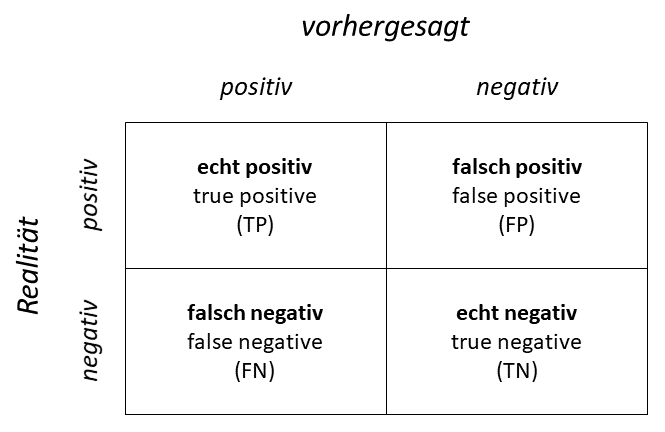
\includegraphics[width=0.7\textwidth]{images/Confusion}
    \caption{allgemeine Konfusionsmatrix\label{fig:confu}}
\end{figure}

Das zum Training der Klassifikatoren verwendete Werkzeug WEKA besitzt die Option, Konfusionsmatrizen zu den durchgeführten Tests der Klassifikatoren auszugeben. Anhand der Werte der Zuordnungen zu den zuvor genannten Gruppen wurden die folgenden Evaluationsmetriken berechnet: 

\begin{itemize}
\item Treffergenauigkeit (Accuracy)
\\Dieser Wert misst die Treffergenauigkeit der Vorhersagen des Klassifikators und gibt an, inwieweit dessen Vorhersagen mit der modellierten Realität übereinstimmen \cite{Sammut2017}. Die Formel zur Berechnung der Accuracy lautet:
\\\[Accuracy = \frac{TP+TN}{TP+TN+FP+FN}\]
Das Ergebnis der Berechnung ist ein prozentualer Wert. 100\% stellen damit die bestmögliche Accuracy dar.
\item Echt-Positiv-Rate / Trefferquote (TP-Rate / Recall)
\\Dieser Wert gibt den Anteil der korrekt als positiv gewerteten Vorhersagen sämtlicher als positiv gewerteter Vorhersagen an \cite{Alpaydin2010}. Die Formel zur Berechnung der TP-Rate bzw. des Recalls lautet:
\\\[TP-Rate = \frac{TP}{TP+FN}\]
Das Ergebnis der Berechnung ist ein prozentualer Wert. 100\% stellen damit die bestmögliche TP-Rate bzw. den bestmöglichen Recall dar. Beide Begriffe werden parallel für die Berechnung der gezeigten Formel verwendet.
\item Positiver Vorhersagewert (Precision)
\\ Dieser Wert gibt die Anzahl der positiven Vorhersagen an, die auch tatsächlich zur positiven Klasse gehören \cite{Sammut2017}. Die Formel zur Bestimmung der Precision lautet:
\\\[Precision = \frac{TP}{TP+FP}\]
Das Ergebnis der Berechnung ist ein prozentualer Wert. 100\% stellen damit die bestmögliche Precision dar.
\item F-Maß (F-Score)
\\ Dieser Wert berechnet das harmonische Mittel der Werte Precision und Recall und liegt somit zwischen diesen beiden Werten, jedoch näher am kleineren Wert \cite{Sammut2017}. Die Formel zur Berechnung des F-Scores lautet:
\\\[F-Score = \frac{2TP}{2TP+FP+FN}\]
Das Ergebnis der Berechnung ist ein prozentualer Wert. 100\% stellen damit den bestmöglichen F-Score dar.
\end{itemize}

\label{roc-def}
Darüber hinaus wurden die sogenannten ROC-Kurven (ROC curve) der einzelnen Klassifikatoren ermittelt. Diese Wahrscheinlichkeitskurven bzw. -graphen (ROC = Receiver Operating characteristic, Betriebsverhalten des Empfängers), beschreiben das Verhältnis zwischen der TP-Rate (y-Achse) und der FP-Rate (x-Achse) \cite{Sammut2017,Narkhede2018}. Die Falsch-Positiv-Rate (FP-Rate) gibt dabei den Anteil der fälschlicherweise als positiv gewerteten Vorhersagen an \cite{Alpaydin2010}. Sie wird mittels der folgenden Formel berechnet:
\\\[FP-Rate = \frac{FP}{FP+TN}\]

Wie bei allen Metriken ist das Ergebnis der FP-Rate ein prozentualer Wert, der bestenfalls möglichst gering ausfallen sollte. Sowohl die TP-Rate als auch die FP-Rate geben nur singuläre Werte an, aus welchen sich keine Graphen herleiten lassen. Jeder Klassifikator errechnet jedoch im Rahmen der Vorhersage eines Datensatzes Wahrscheinlichkeiten, die die Zugehörigkeit zu den Werten der Zielklasse darstellen \cite{KNIMETV2019}. In der Regel wird ein Datenpunkt der positiven Klasse zugeordnet, wenn die Wahrscheinlichkeit einen Schwellenwert von 0,5 übersteigt - Datenpunkte, die diesen Schwellenwert unterschreiten werden wiederum der negativen Klasse zugeordnet \cite{KNIMETV2019}. Wird der Schwellenwert erhöht, so werden weniger Datenpunkte der positiven Klasse zugeordnet, wohingegen im Falle einer Absenkung des Schwellenwertes mehr Datenpunkte der positiven Klasse zugeordnet werden \cite{KNIMETV2019}. Für die Erstellung der ROC-Kurven werden somit die Werte der TP-Rate und der FP-Rate unter der Berücksichtigung der Schwellenwerte im Bereich von 0,0 bis 1,0 gegenübergestellt.

Eine weitere Metrik, die in Verbindung mit der ROC-Kurve auftritt, ist der ROC-Bereich (ROC area). Dieser Wert, der anhand der ROC-Kurve berechnet wird und auch AUC-Bereich (AUC = Area Under Curve, Bereich unter der Kurve) genannt wird, gibt an, in wieweit ein Klassifikator in der Lage ist, zwischen den Werten der Zielklassen zu unterscheiden \cite{Narkhede2018}. Je höher dieser Wert ist (1,0 ist das Maximum), desto besser trifft der Klassifikator korrekte Vorhersagen \cite{Narkhede2018}.

Am Beispiel des Schwellenwertes 0,5 wird nun die Interpretation der ROC-Kurve und des ROC-Bereiches vorgenommen. Unterstützt wird dies durch grafische Beispiele, die in \autoref{fig:curves} gezeigt werden. Der Idealfall ist in (a) und (b) dargestellt. Die Wahrscheinlichkeitskurven der Zielklasse (a) weisen keine Überlappung auf. Die Werte der Zielklasse sind somit allesamt korrekt zugeordnet worden, sodass der Klassifikator korrekt zwischen diesen unterscheiden kann. Die diesem Fall entsprechende ROC-Kurve ist in (b) dargestellt. Der ROC-Bereich beträt in diesem Fall 1,0. Ein \glqq Normalfall\grqq{} ist in (c) und (d) dargestellt. Es ist in (c) zu erkennen, dass die Wahrscheinlichkeitskurven überlappen, sodass falsche Zuordnungen getroffen werden. Die entsprechende ROC-Kurve ist in (d) dargestellt. Der entsprechende ROC-Bereich beträgt im hier gezeigten Fall 0,7. Dies bedeutet, dass 70\% der Zuordnungen richtig getroffen werden. Verbessert werden können die Werte möglicherweise, wenn der Schwellenwert verändert wird. Der \glqq Worst Case\grqq, der bei der Performanzmessung mittels ROC-Kurven auftreten kann, ist in (e) und (f) dargestellt. In (e) ist zu erkennen, dass sich die Wahrscheinlichkeitskurven vollständig überlappen. Es findet somit eine willkürliche Zuordnung statt. Die zugehörige ROC-Kruve (f) entspricht einer Winkelhalbierenden. Ein weiterer Fehlerfall ist in (g) und (h) dargestellt. Die Wahrscheinlichkeitskurven (g) zeigen, dass die Zuordnungen gegenteilig erfolgen und somit der jeweils dem anderen Wert der Zielklasse falsch zugeordnet werden. Der entsprechende ROC-Bereich beträgt 0, da wie in (h) zu sehen ist, keine Fläche unter der Kurve vorhanden ist.

\begin{figure}[ht]
  \centering
  \subfloat[][Idealfall]{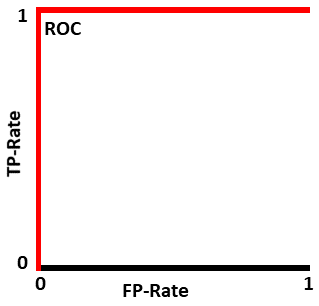
\includegraphics[width=0.5\linewidth]{images/roc_ideal}}
  \subfloat[][Idealfall]{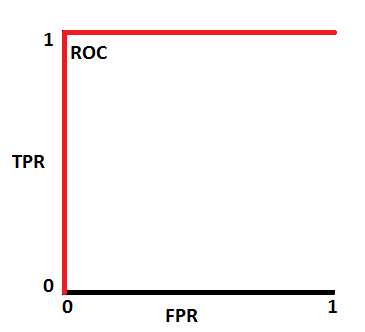
\includegraphics[width=0.25\linewidth]{images/roc_ideal_curve}}
  \qquad
  \subfloat[][\glqq Normalfall\grqq]{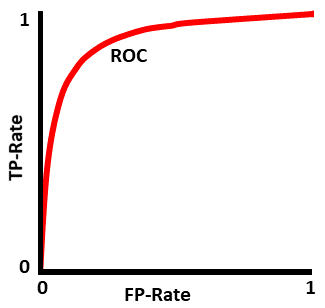
\includegraphics[width=0.5\linewidth]{images/roc_normal}}
  \subfloat[][\glqq Normalfall\grqq]{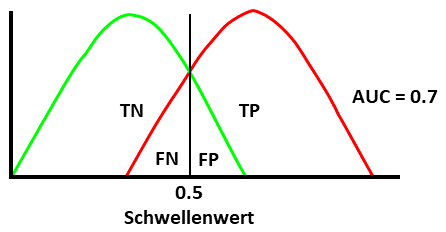
\includegraphics[width=0.25\linewidth]{images/roc_normal_curve}}
  \qquad
  \subfloat[][\glqq Worst Case\grqq]{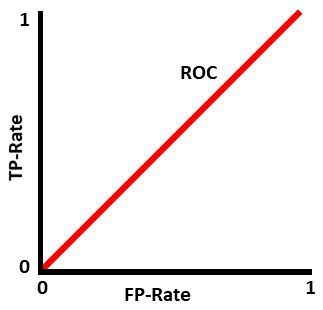
\includegraphics[width=0.5\linewidth]{images/roc_worst}}
  \subfloat[][\glqq Worst Case\grqq]{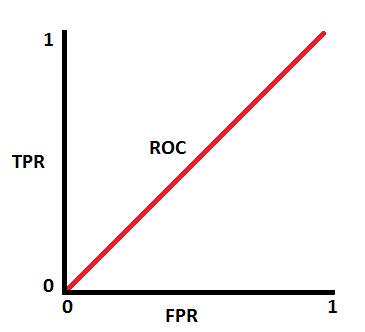
\includegraphics[width=0.25\linewidth]{images/roc_worst_curve}}
  \qquad
  \subfloat[][Fehlerfall]{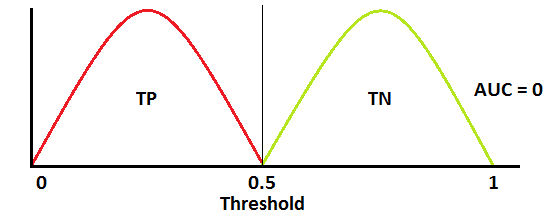
\includegraphics[width=0.5\linewidth]{images/roc_neg}}
  \subfloat[][Fehlerfall]{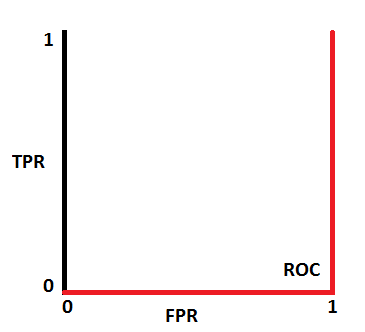
\includegraphics[width=0.25\linewidth]{images/roc_neg_curve}}
  \caption{Beispiel zur Interpretation der ROC-Kurve und des ROC-Bereiches (TPR = TP-Rate, FPR = FP-Rate, Threshold = Schwellenwert) \cite{Narkhede2018}
\label{fig:curves}}
\end{figure}

Alle vorgestellten Metriken werden automatisiert von WEKA berechnet. Ferner besitzt das Werkzeug die Fähigkeit, ROC-Kurven mit den entsprechenden ROC-Werten auszugeben. Die im Rahmen der Evaluation der Klassifikatoren ermittelten Werte der Metriken sowie die ROC-Kurven und Werte der ROC-Bereiche werden im folgenden Abschnitt aufgeführt sowie verglichen und interpretiert.

\fbox{\parbox{\linewidth}{RQ3a: WELCHE MITEINANDER VERGLEICHBAREN MERKMALE BESITZEN DIE KLASSIFIKATOREN?\medskip\\
Die Merkmale zum Vergleich stellen Evaluationsmetriken dar, welche auf Basis der Ergebnisse des Tests der Klassifikatoren errechnet werden und die Performanz der Vorhersagen auf verschiedene Weisen messen. Welche Metriken berechnet wurden beantwortet Forschungsfrage RQ3b.}}

\fbox{\parbox{\linewidth}{RQ3b: WELCHE METRIKEN KÖNNEN FÜR DEN VERGLEICH VERWENDET WERDEN?\medskip\\
Für den Vergleich der Klassifikatoren werden klassische Evaluationsmetriken verwendet, welche auf Basis von Konfusionsmatrizen berechnet werden. Die betrachteten Metriken lauten: Accuracy, TP-Rate / Recall, Precision und F-Score. Ebenfalls hinzugezogen werden die jeweiligen ROC-Kurven der Klassifikatoren inklusive der ROC-Bereiche. Diese Metriken stellen einen Standard für die Messung der Performanz der Vorhersagen von Klassifikatoren dar.}}

\section{Ergebnisse und Diskussion}
\label{results}

Dieser Abschnitt umfasst die Ergebnisse und vergleichenden Diskussionen zu den Tests der Klassifikatoren der drei Datensets, aufgeteilt in einen Unterabschnitt für das featurebasierte Datenset und einen Abschnitt für die dateibasierten Datensets. Darüber hinaus sind die Unterabschnitte wie folgt aufgeteilt: Konfusionsmatrizen, Accuracies, weitere Evaluationsmetriken, ROC-Kurven und ROC-Bereiche sowie Zusammenfassung.

\subsection{Featurebasiertes Datenset}

Die Präsentation der Ergebnisse beginnt mit denen des featurebasierten Datensets.

\subsubsection*{Konfusionsmatrizen}

Die Konfusionsmatrizen dienen als Basis der Ergebnisse der Evaluation der Klassifikatoren anhand der zuvor vorgestellten Metriken. Die Matrizen des featurebasierten Datensets sind in \autoref{tab:mat-feat} aufgeführt. Dabei bilden die Spalten die von den Klassifikatoren vorhergesagten Label ab. Die Zeilen bilden wiederum die \glqq ground truth\grqq{}, also die im Rahmen der Erstellung der Datensets ermittelte Realität, ab. Außerdem werden die ermittelten Werte der jeweiligen Klassen in den Spalten \glqq total\grqq zusammengezählt. Da für jeden Klassifikator das selbe Testset gewählt wurde, sind die Werte der \glqq total\grqq-Spalte identisch. Die für die Klassifikatoren verwendeten Abkürzungen können \autoref{tab:classifiers} entnommen werden.

\begin{table}[ht]
\centering
\caption{Konfusionsmatrizen des featurebasierten Datensets}
\label{tab:mat-feat}
\resizebox{\linewidth}{!}{%
\begin{tabular}{|>{\hspace{0pt}}p{0.119\linewidth}>{\hspace{0pt}}p{0.362\linewidth}|>{\RaggedLeft\hspace{0pt}}p{0.156\linewidth}>{\RaggedLeft\hspace{0pt}}p{0.214\linewidth}>{\RaggedLeft\hspace{0pt}}p{0.139\linewidth}|} 
\cline{2-5}
\multicolumn{1}{>{\Centering\hspace{0pt}}p{0.119\linewidth}|}{} & \textbf{Ermittelt -\textgreater{}} & \textbf{defekt}  & \textbf{fehlerfrei}  & \textbf{total}  \\ 
\hline
\multirow{3}{0.119\linewidth}{\hspace{0pt}J48}                  & Realität defekt                    & 446              & 320                  & 766             \\
                                                                & Realität fehlerfrei                & 483              & 3.142                & 3.625           \\
                                                                & total                              & 929              & 3.462                & 4.391           \\ 
\hline
\multirow{3}{0.119\linewidth}{\hspace{0pt}KNN}                  & Realität defekt                    & 371              & 395                  & 766             \\
                                                                & Realität fehlerfrei                & 569              & 3.056                & 3.625           \\
                                                                & total                              & 940              & 3.451                & 4.391           \\ 
\hline
\multirow{3}{0.119\linewidth}{\hspace{0pt}LR}                   & Realität defekt                    & 309              & 457                  & 766             \\
                                                                & Realität fehlerfrei                & 1.020            & 2.605                & 3.625           \\
                                                                & total                              & 1.329            & 3.061                & 4.391           \\ 
\hline
\multirow{3}{0.119\linewidth}{\hspace{0pt}NB}                   & Realität defekt                    & 322              & 444                  & 766             \\
                                                                & Realität fehlerfrei                & 265              & 3.360                & 3.625           \\
                                                                & total                              & 587              & 3.804                & 4.391           \\ 
\hline
\multirow{3}{0.119\linewidth}{\hspace{0pt}NN}                   & Realität defekt                    & 327              & 439                  & 766             \\
                                                                & Realität fehlerfrei                & 1.019            & 2.606                & 3.625           \\
                                                                & total                              & 1.346            & 3.045                & 4.391           \\ 
\hline
\multirow{3}{0.119\linewidth}{\hspace{0pt}RF}                   & Realität defekt                    & 504              & 262                  & 766             \\
                                                                & Realität fehlerfrei                & 450              & 3.175                & 3.625           \\
                                                                & total                              & 954              & 3.437                & 4.391           \\ 
\hline
\multirow{3}{0.119\linewidth}{\hspace{0pt}SGD}                  & Realität defekt                    & 251              & 515                  & 766             \\
                                                                & Realität fehlerfrei                & 938              & 2.687                & 3.625           \\
                                                                & total                              & 1.189            & 3.202                & 4.391           \\ 
\hline
\multirow{3}{0.119\linewidth}{\hspace{0pt}SVM}                  & Realität defekt                    & 176              & 590                  & 766             \\
                                                                & Realität fehlerfrei                & 899              & 2.726                & 3.625           \\
                                                                & total                              & 1.075            & 3.316                & 4.391           \\
\hline
\end{tabular}
}
\end{table}

\subsubsection*{Accuracies}

Die erste Metrik, die verglichen wird, ist die Accuracy. Diese gibt die Treffergenauigkeit der Klassifikatoren an. Dargestellt werden die Ergebnisse zum besseren Vergleich als Balkendiagramme. Das Diagramm des feturebasierten Datensets ist in \autoref{fig:final-feat} dargestellt. Die konkreten Zahlenwerte können im \hyperref[appendix2]{Anhang} eingesehen werden.

\begin{figure}[ht]
    \centering
    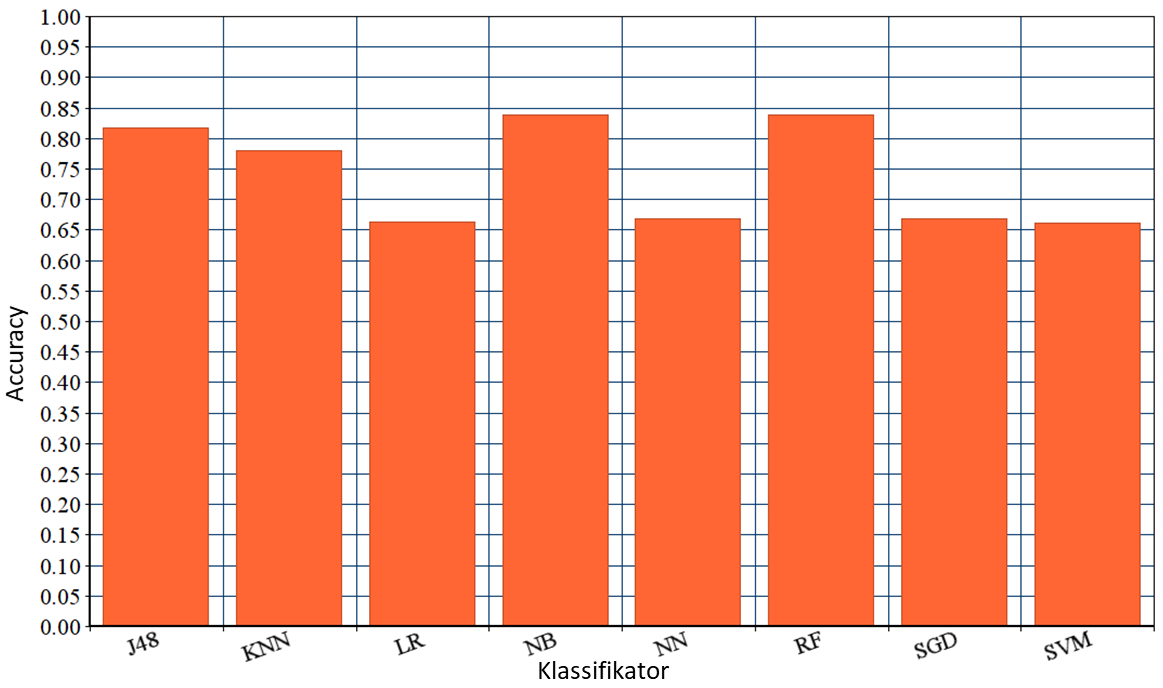
\includegraphics[width=\textwidth]{images/final_feat}
    \caption{Vergleich der Accuracies des featurebasierten Datensets\label{fig:final-feat}}
\end{figure}

Die Ergebnisse zeigen, dass die Accuracies der Klassifikatoren zwischen 66\% und 84\% liegen. Die höchsten Werte erreichten die Klassifikatoren NB und RF mit einer Treffergenauigkeit von jeweils 84\%. Mit einem Wert von 82\% erreichte auch der J48-Klassifikator eine überdurchschnittlich hohe Performanz. Darauf folgt der KNN-Klassifikator mit 78\%. Mit Werten von 66\% beziehungsweise 67\% schnitten die Klassifikatoren LR, NN, SGD und SVM am schlechtesten ab. Sie ermitteln somit in über 30\% der Vorhersagen ein falsches Ergebnis. Auffällig an diesen Ergebnissen ist die hohe Performanz beider Entscheidungsbaum-basierter Klassifikatoren J48 und RF. Sie scheinen somit die Eingabemenge am besten verarbeiten zu können, um Rückschlüsse auf die neuen Daten in Form der Testdaten schließen zu können.

\subsubsection*{Weitere Evaluationsmetriken}

Dieser Abschnitt stellt die Ergebnisse der weiteren Evaluationsmetriken TP-Rate / Recall, FP-Rate, Precision und F-Score vor. Diese können in \autoref{tab:met-results-feat} für das featurebasierte Datenset eingesehen werden. Aufgeteilt werden die Ergebnisse nach den Werten der Zielklasse \glqq defekt\grqq{} und \glqq fehlerfrei\grqq. Zudem wird der Mittelwert der Ergebnisse beider Werte der Zielklasse angegeben. Er zeigt die Performanz aggregiert für beide Werte an und liegt im Idealfall bei 1,00. Die vollständigen Tabellen der Ergebnisse der Evaluation, inklusive einer weiteren Metrik, können im \hyperref[appendix3]{Anhang} gefunden werden.

\begin{table}[ht]
\centering
\caption{Ergebnisse der Evaluationsmetriken des featurebasierten Datensets}
\label{tab:met-results-feat}
\resizebox{\linewidth}{!}{%
\begin{tabular}{|>{\hspace{0pt}}p{0.12\linewidth}>{\hspace{0pt}}p{0.349\linewidth}|>{\RaggedLeft\hspace{0pt}}p{0.156\linewidth}>{\RaggedLeft\hspace{0pt}}p{0.214\linewidth}>{\RaggedLeft\hspace{0pt}}p{0.141\linewidth}|} 
\cline{3-5}
\multicolumn{1}{>{\hspace{0pt}}p{0.12\linewidth}}{} &                  & \textbf{defekt}  & \textbf{fehlerfrei}  & \textbf{Mittel}   \\ 
\hline
\multirow{4}{0.12\linewidth}{\hspace{0pt}J48}       & TP-Rate / Recall & 0,58             & 0,87                 & 0,73              \\
                                                    & FP-Rate          & 0,13             & 0,42                 & 0,28              \\
                                                    & Precision        & 0,48             & 0,91                 & 0,70              \\
                                                    & F-Score          & 0,53             & 0,89                 & 0,71              \\ 
\hline
\multirow{4}{0.12\linewidth}{\hspace{0pt}KNN}       & TP-Rate / Recall & 0,48             & 0,86                 & 0,67              \\
                                                    & FP-Rate          & 0,16             & 0,52                 & 0,68              \\
                                                    & Precision        & 0,40             & 0,89                 & 0,65              \\
                                                    & F-Score          & 0,44             & 0,86                 & 0,66              \\ 
\hline
\multirow{4}{0.12\linewidth}{\hspace{0pt}LR}        & TP-Rate / Recall & 0,40             & 0,72                 & 0,56              \\
                                                    & FP-Rate          & 0,28             & 0,60                 & 0,44              \\
                                                    & Precision        & 0,23             & 0,85                 & 0,54              \\
                                                    & F-Score          & 0,30             & 0,78                 & 0,54              \\ 
\hline
\multirow{4}{0.12\linewidth}{\hspace{0pt}NB}        & TP-Rate / Recall & 0,42             & 0,93                 & 0,68              \\
                                                    & FP-Rate          & 0,07             & 0,58                 & 0,33              \\
                                                    & Precision        & 0,55             & 0,88                 & 0,72              \\
                                                    & F-Score          & 0,48             & 0,91                 & 0,70              \\ 
\hline
\multirow{4}{0.12\linewidth}{\hspace{0pt}NN}        & TP-Rate / Recall & 0,43             & 0,72                 & 0,58              \\
                                                    & FP-Rate          & 0,28             & 0,57                 & 0,43              \\
                                                    & Precision        & 0,24             & 0,86                 & 0,55              \\
                                                    & F-Score          & 0,31             & 0,78                 & 0,55              \\ 
\hline
\multirow{4}{0.12\linewidth}{\hspace{0pt}RF}        & TP-Rate / Recall & 0,66             & 0,88                 & 0,77              \\
                                                    & FP-Rate          & 0,12             & 0,34                 & 0,23              \\
                                                    & Precision        & 0,53             & 0,92                 & 0,73              \\
                                                    & F-Score          & 0,59             & 0,90                 & 0,75              \\ 
\hline
\multirow{4}{0.12\linewidth}{\hspace{0pt}SGD}       & TP-Rate / Recall & 0,34             & 0,74                 & 0,54              \\
                                                    & FP-Rate          & 0,56             & 0,67                 & 0,62              \\
                                                    & Precision        & 0,21             & 0,84                 & 0,53              \\
                                                    & F-Score          & 0,26             & 0,79                 & 0,53              \\ 
\hline
\multirow{4}{0.12\linewidth}{\hspace{0pt}SVM}       & TP-Rate / Recall & 0,23             & 0,75                 & 0,48              \\
                                                    & FP-Rate          & 0,25             & 0,77                 & 0,51              \\
                                                    & Precision        & 0,16             & 0,82                 & 0,49              \\
                                                    & F-Score          & 0,19             & 0,79                 & 0,49              \\
\hline
\end{tabular}
}
\end{table}

Eine erste Betrachtung der Ergebnisse der Evaluationsmetriken zeigt, dass die Resultate (mit Ausnahme der FP-Rate) bezogen auf das Label \glqq defekt\grqq{} schlechter ausfallen, als die des Labels \glqq fehlerfrei\grqq. Die im Vergleich besten Ergebnisse wurden vom RF-Klassifikator für das Label \glqq defekt\grqq{} erreicht. 66\% der tatsächlich defekten Datensätze wurden auch als solche vorhergesagt und lediglich 12\% der Datensätze wurden hingegen fälschlicherweise als defekt vorhergesagt. Die Werte der Precision und des F-Scores liegen bei 53\% respektive 59\% auf einem durchschnittlichen Niveau. Vergleichbare Ergebnisse erzielte der J48-Klassifikator. Die insgesamt schlechtesten Werte weisen SGD und SVM auf. Ihre Genauigkeit der Erkennung der tatsächlich defekten Datensätze betragen nur 34\% beziehungsweise 23\%. Die weiteren Klassifikatoren operierten auf einem durchschnittlichen Level.

Die jeweiligen Mittelwerte können betrachtet werden, um die Gesamtperformanz der Klassifikatoren für beide Label zu vergleichen. Hier schneidet erneut der RF-Klassifikator am besten ab. Die Werte für die TP-Rate, die Precision und den F-Score liegen im Umfeld von über 73\% und sind damit vergleichsweise überdurchschnittlich hoch. Die FP-Rate in Höhe von 23\%, die hauptsächlich durch die Ergebnisse hinsichtlich des Labels \glqq fehlerfrei\grqq{} geschuldet ist, liegt auf dem niedrigsten Niveau aller Klassifikatoren. Erneut sind die Ergebnisse des ebenfalls Entscheidungsbaum-basierten Klassifikators J48 auf einem ähnlichen Niveau. Die Klassifikatoren KNN und NB weisen durch ihre hohen Werte der FP-Rate insgesamt durchschnittliche Performanz auf. In der Gesamtheit betrachtet zeigen die Werte der Klassifikatoren LR, NN, SGD und SVM, dass diese im Vergleich die schlechteste Performanz besitzen. Insbesondere die FP-Raten von über 43\% sind auf einem hohen, nicht wünschenswerten Niveau. 

\subsubsection*{ROC-Kurven und ROC-Bereiche}

Die Interpretation der ROC-Kurven und ROC-Bereiche erfolgt anhand des in \hyperref[roc-def]{Abschnitt 5.2.1} vorgestellten Schemas. Die ROC-Kurven samt der Werte der ROC-Bereiche (repräsentiert durch \glqq AUC\grqq{}) sind in \autoref{fig:roc-feat}  dargestellt. Zu sehen sind jeweils die von WEKA ausgegebenen und unveränderten Plots. Die dargestellten Farbverläufe der Kurven verdeutlichen keine für diesen Zweck relevanten Informationen und können somit ignoriert werden.

\begin{figure}[ht]
  \centering
  \subfloat[][J48\\AUC = 0,77]{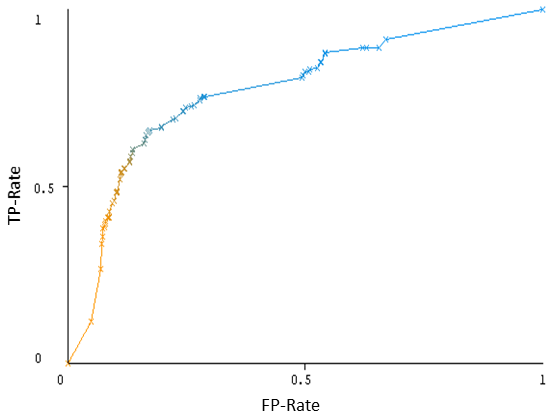
\includegraphics[width=0.25\linewidth]{images/j48_feat}} 
  \subfloat[][LR\\AUC = 0,62]{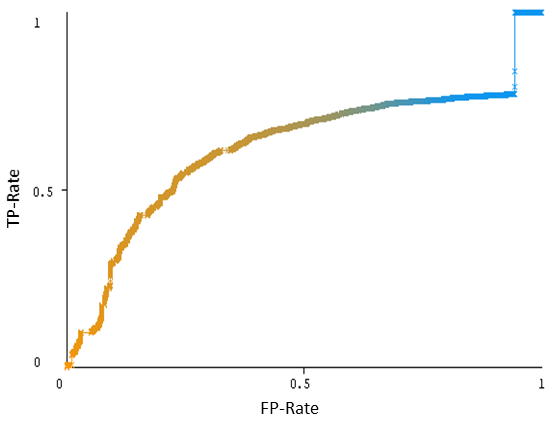
\includegraphics[width=0.25\linewidth]{images/lr_feat}}
  \subfloat[][NN\\AUC = 0,61]{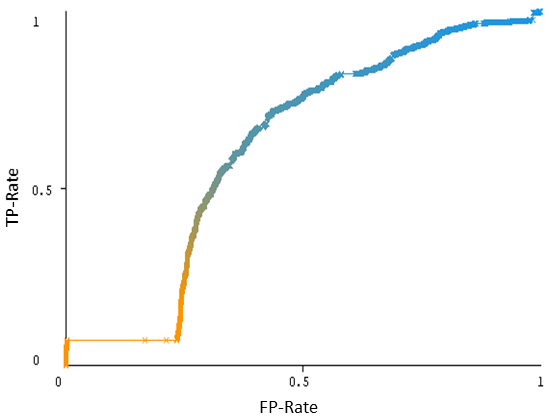
\includegraphics[width=0.25\linewidth]{images/nn_feat}}
  \subfloat[][SGD\\AUC = 0,53]{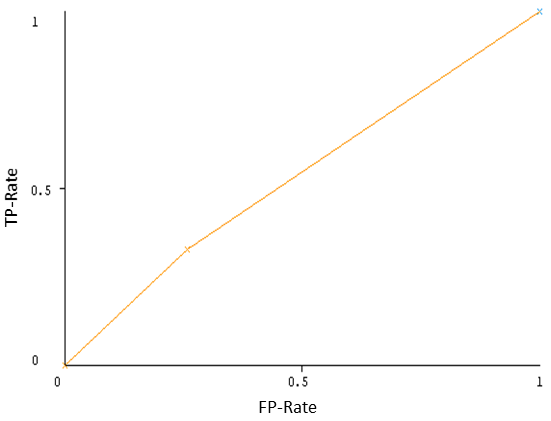
\includegraphics[width=0.25\linewidth]{images/sgd_feat}}
  \qquad
  \subfloat[][KNN\\AUC = 0,73]{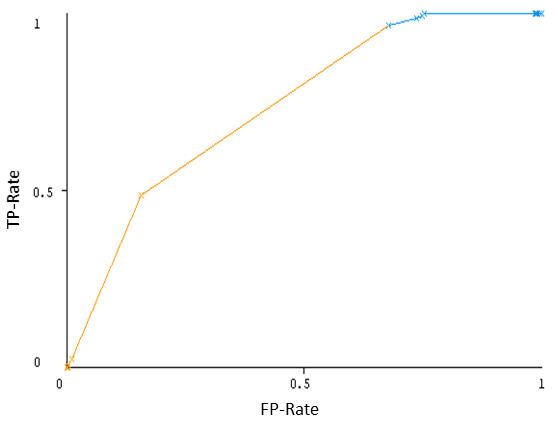
\includegraphics[width=0.25\linewidth]{images/knn_feat}}
  \subfloat[][NB\\AUC = 0,80]{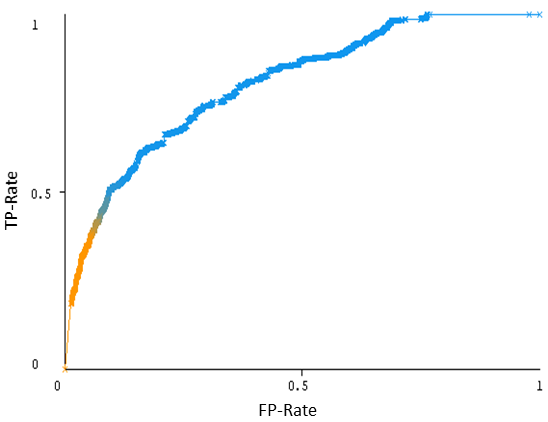
\includegraphics[width=0.25\linewidth]{images/nb_feat}}
  \subfloat[][RF\\AUC = 0,84]{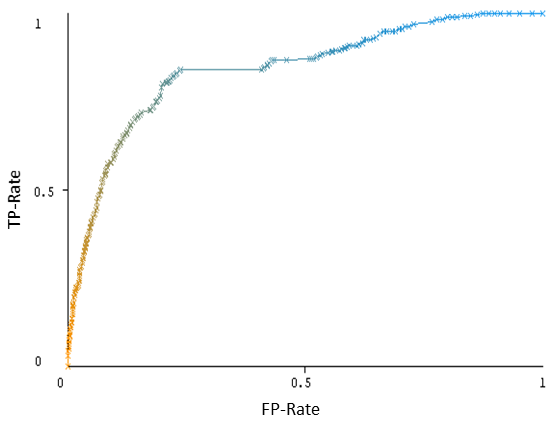
\includegraphics[width=0.25\linewidth]{images/rf_feat}} 
  \subfloat[][SVM\\AUC = 0,49]{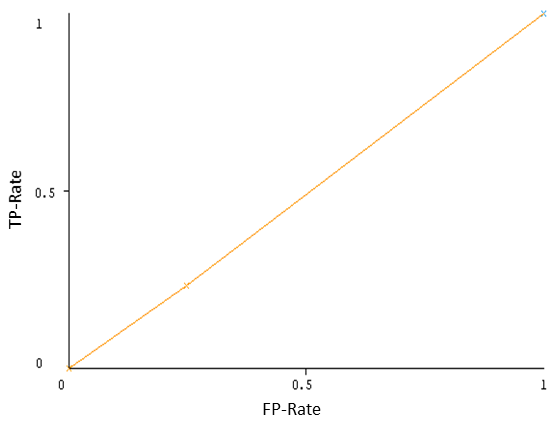
\includegraphics[width=0.25\linewidth]{images/svm_feat}}
  \caption{ROC-Kurven des featurebasierten Datensets \label{fig:roc-feat}}
\end{figure}

Es ist zu erkennen, dass keine ROC-Kurve den in \hyperref[roc-def]{Abschnitt 5.2.1} vorgestellten Idealfall annähert. Die beste Vorhersageperformanz zeigt erneut der RF-Klassifikator mit einem ROC-Bereich von 0,84. Der NB-Klassifikator zeigt eine minimal geringere Performanz mit einem ROC-Bereich von 0,80. Eine durchschnittliche Performanz von 0,77 beziehungsweise 0,72, bezogen auf den ROC-Bereich, weisen die Klassifikatoren J48 und KNN auf. Die Performanz der LR- und NN-Klassifikatoren liegen im unteren Durchschnitt. Den unerwünschten Fall einer winkelhalbierenden ROC-Kurve zeigen die SGD- und SVM-Klassifikatoren. Dies spiegeln auch die ROC-Bereiche wider. Sie \glqq raten\grqq{} somit, statt präzise Vorhersagen zu treffen.

\subsubsection*{Zusammenfassung}
In jeder der betrachteten Kategorien von Metriken erwiesen sich die Entscheidungsbaum-bas-ierten Klassifikatoren J48 und RF als am performantesten im Vergleich zu den weiteren Klassifikatoren. Der RF-Klassifikator erreichte dabei meist zudem eine etwas höhere Performanz. Die den Klassifikatoren zugrundeliegenden Algorithmen scheinen das gegebene featurebasierte Datenset mit seinen elf Attributen am besten hinsichtlich der Entwicklung der Ableitungsfunktion zur Vorhersage neuer Daten am besten verarbeiten zu können.
Die Klassifikatoren SGD und SVM zeigten für jede Kategorie von Evaluationsmetriken stets die im Vergleich schlechtesten Performanzen. Es wurde zudem festgestellt, dass die Klassifikatoren raten, statt Vorhersagen zu treffen. Das featurebasierte Datenset scheint somit für diese Klassifikationsalgorithmen nicht geeignet zu sein. Gründe dafür können eine zu geringe Anzahl an Instanzen oder eine zu hohe Anzahl an Attributen sein.

\subsection{Dateibasierter Vergleich}
\label{classic-eval}

Dieser Abschnitt dient zur Evaluation und zum Vergleich der dateienbasierten Datensets, deren Erstellung in \hyperref[new-datasets]{Abschnitt 3.3} erläutert wurde. Der Grund dieses Vergleiches ist die Messung der Einflüsse der featurebasierten Metriken auf die Vorhersagen einer klassischen dateibasierten Methode, die der wissenschaftlichen Literatur entnommen wurde \cite{Moser2008}. Die Aufteilung dieses Abschnitts ist analog zum vorherigen Abschnitt.

\subsubsection*{Konfusionsmatrizen}

Die Konfusionsmatrizen der dateibasierten Datensets sind in \autoref{tab:mat-eval} aufgeführt. Die übergeordneten Spalten sind dabei in das \glqq einfache\grqq{} und das erweiterte Datenset angeordnet. Beide Datensets umfassen die selbe Anzahl an Datensätzen, somit sind die \glqq total\grqq -Spalten identisch.
Eine kurze Analyse der \glqq defekt\grqq - \glqq Realität defekt\grqq - Felder zeigt, dass nur sehr wenige tatsächlich defekten Datensätze auch wirklich als defekt vorhergesagt wurden. Dies wird sich auch in den weiteren Ergebnissen der Evaluationsmetriken widerspiegeln.

\begin{table}[ht]
\centering
\caption{Konfusionsmatrizen der dateibasierten Datensets}
\label{tab:mat-eval}
\resizebox{\linewidth}{!}{%
\begin{tabular}{|>{\hspace{0pt}}p{0.075\linewidth}>{\hspace{0pt}}p{0.231\linewidth}|>{\RaggedLeft\hspace{0pt}}p{0.1\linewidth}>{\RaggedLeft\hspace{0pt}}p{0.135\linewidth}>{\RaggedLeft\hspace{0pt}}p{0.1\linewidth}|>{\RaggedLeft\hspace{0pt}}p{0.102\linewidth}>{\RaggedLeft\hspace{0pt}}p{0.137\linewidth}>{\RaggedLeft\hspace{0pt}}p{0.104\linewidth}|} 
\cline{3-8}
\multicolumn{1}{>{\hspace{0pt}}p{0.075\linewidth}}{}            &                                    & \multicolumn{3}{>{\Centering\hspace{0pt}}p{0.335\linewidth}|}{\textbf{\glqq einfaches\grqq{} dateibasiertes Datenset}} & \multicolumn{3}{>{\Centering\hspace{0pt}}p{0.343\linewidth}|}{\textbf{erweitertes dateibasiertes Datenset}}  \\ 
\cline{2-8}
\multicolumn{1}{>{\Centering\hspace{0pt}}p{0.075\linewidth}|}{} & \textbf{Ermittelt -\textgreater{}} & \textbf{defekt} & \textbf{fehlerfrei} & \textbf{total}                                & \textbf{defekt} & \textbf{fehlerfrei} & \textbf{total}                                        \\ 
\hline
\multirow{3}{0.075\linewidth}{\hspace{0pt}J48}                   & Realität defekt                    & 11              & 102                 & 113                                           & 15              & 98                  & 113                                                   \\
                                                                & Realität fehlerfrei                & 911             & 20.923              & 21.834                                        & 1.120           & 20.714              & 21.834                                                \\
                                                                & total                              & 922             & 21.025              & 21.947                                        & 1.135           & 2.0812              & 21.947                                                \\ 
\hline
\multirow{3}{0.075\linewidth}{\hspace{0pt}KNN}                  & Realität defekt                    & 29              & 84                  & 113                                           & 20              & 93                  & 113                                                   \\
                                                                & Realität fehlerfrei                & 5.209           & 16.625              & 21.834                                        & 4.861           & 16.973              & 21.834                                                \\
                                                                & total                              & 5.238           & 16.709              & 21.947                                        & 4.881           & 17.066              & 21.947                                                \\ 
\hline
\multirow{3}{0.075\linewidth}{\hspace{0pt}LR}                   & Realität defekt                    & 36              & 77                  & 113                                           & 32              & 81                  & 113                                                   \\
                                                                & Realität fehlerfrei                & 2.520           & 19.314              & 21.834                                        & 2.578           & 19.256              & 21.834                                                \\
                                                                & total                              & 2.556           & 19.391              & 21.947                                        & 2.610           & 19.337              & 21.947                                                \\ 
\hline
\multirow{3}{0.075\linewidth}{\hspace{0pt}NB}                   & Realität defekt                    & 77              & 36                  & 113                                           & 83              & 30                  & 113                                                   \\
                                                                & Realität fehlerfrei                & 18.700          & 3.134               & 21.834                                        & 18.750          & 3.084               & 21.834                                                \\
                                                                & total                              & 18.777          & 3.170               & 21.947                                        & 18.833          & 3.114               & 21.947                                                \\ 
\hline
\multirow{3}{0.075\linewidth}{\hspace{0pt}NN}                   & Realität defekt                    & 6               & 107                 & 113                                           & 1               & 112                 & 113                                                   \\
                                                                & Realität fehlerfrei                & 4.341           & 17.493              & 21.834                                        & 141             & 21.693              & 21.834                                                \\
                                                                & total                              & 4.347           & 17.600              & 21.947                                        & 142             & 21.805              & 21.947                                                \\ 
\hline
\multirow{3}{0.075\linewidth}{\hspace{0pt}RF}                   & Realität defekt                    & 7               & 106                 & 113                                           & 4               & 109                 & 113                                                   \\
                                                                & Realität fehlerfrei                & 382             & 21.452              & 21.834                                        & 366             & 21.468              & 21.834                                                \\
                                                                & total                              & 389             & 21.558              & 21.947                                        & 370             & 21.577              & 21.947                                                \\ 
\hline
\multirow{3}{0.075\linewidth}{\hspace{0pt}SGD}                  & Realität defekt                    & 22              & 91                  & 113                                           & 20              & 93                  & 113                                                   \\
                                                                & Realität fehlerfrei                & 1.260           & 20.574              & 21.834                                        & 1.226           & 20.608              & 21.834                                                \\
                                                                & total                              & 1.282           & 20.665              & 21.947                                        & 1.246           & 20.701              & 21.947                                                \\ 
\hline
\multirow{3}{0.075\linewidth}{\hspace{0pt}SVM}                  & Realität defekt                    & 22              & 91                  & 113                                           & 21              & 92                  & 113                                                   \\
                                                                & Realität fehlerfrei                & 1.041           & 20.793              & 21.834                                        & 991             & 20.843              & 21.834                                                \\
                                                                & total                              & 1.063           & 20.884              & 21.947                                        & 1.012           & 20.935              & 21.947                                                \\
\hline
\end{tabular}
}
\end{table}

\subsubsection*{Accuracies}

Die Accuracies der Klassifikatoren der dateibasierten Datensets sind in \autoref{fig:final-eval} dargestellt. Die konkreten Zahlenwerte können dem \hyperref[appendix2]{Anhang} entnommen werden.

\begin{figure}[ht]
    \centering
    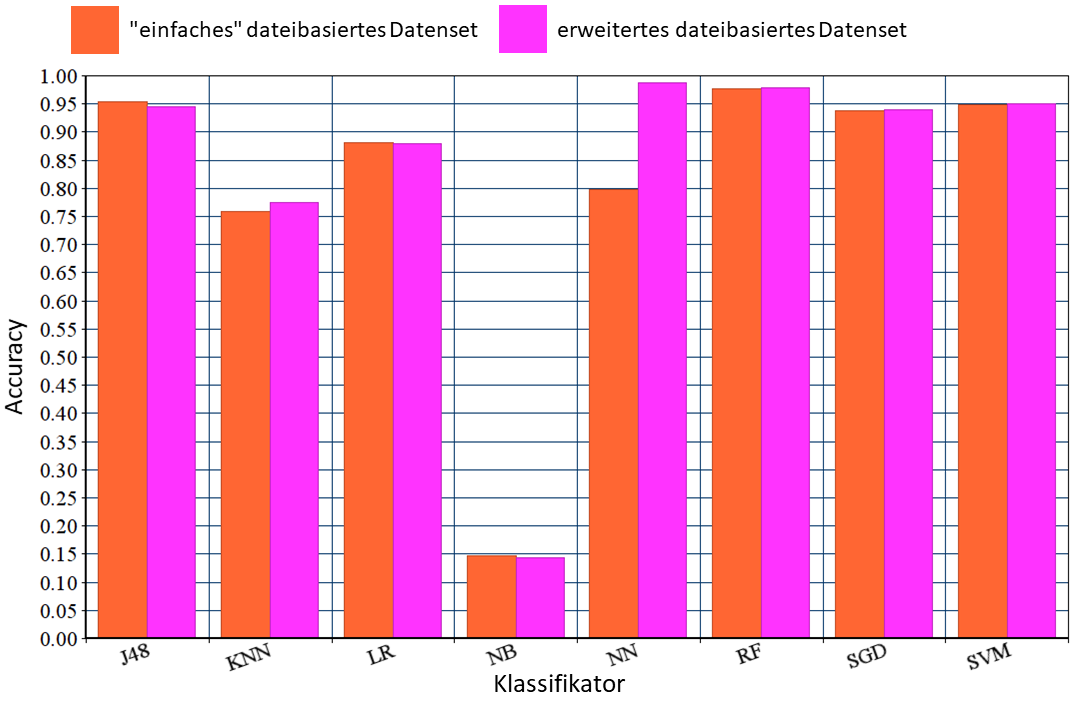
\includegraphics[width=\textwidth]{images/final_eval}
    \caption{Vergleich der Accuracies der dateibasierten Datensets\label{fig:final-eval}}
\end{figure}

Der Vergleich zwischen den Datensets zeigt, dass die Einbindung der featurebasierten Metriken für sechs von acht Klassifikatoren keinen signifikanten Einfluss auf die Performanz der Vorhersagen hat. Die erzielten Werte der Accuracies sind dort jeweils auf dem selben Niveau. Die im Vergleich schlechteste Accuracy erzielt der NB-Klassifikator mit etwa 15\% Treffergenauigkeit. Dieser scheint die hohe Anzahl an Datensätzen nicht korrekt verarbeiten zu können. Die Klassifikatoren KNN und LR erreichten mit etwa 76\% beziehungsweise 87\% überdurchschnittlich hohe Ergebnisse. Mit Werten von über 90\% besitzen die Klassifikatoren J48, RF, SGD und SVM äußerst hohe Werte, deren Aussagekraft zunächst infrage gestellt werden und die weiteren Evaluationsmetriken betrachtet werden sollten.
Eine Auffälligkeit zeigt der NN-Klassifikator. Es ist ein deutlicher Sprung der Werte von etwa 18\% zwischen dem \glqq einfachen\grqq{} und dem erweiterten Datenset zu erkennen. Diese Auffälligkeit sollte ebenfalls anhand der weiteren Evaluationsmetriken analysiert und interpretiert werden. Sie kann einerseits verdeutlichen, dass der Klassifikator des erweiterten Datensets durch die Hinzunahme der zusätzlichen Attribute genauere Vorhersagen treffen kann oder durch diesen Umstand die Vorhersagen negativ beeinflusst werden, sodass die Ergebnisse verzerrt werden.

\subsubsection*{Weitere Evaluationsmetriken}

Dieser Abschnitt stellt die Ergebnisse der weiteren Evaluationsmetriken der dateibasierten Datensets in \autoref{tab:met-results} vor. Die übergeordneten Spalten werden erneut durch die beiden Datensets repräsentiert. Die vollständigen Tabellen der Ergebnisse der Evaluation, inklusive einer weiteren Metrik, können im \hyperref[appendix3]{Anhang} gefunden werden.

\begin{table}
\centering
\caption{Ergebnisse der Evaluationsmetriken der dateibasierten Datensets (TPR = TP-Rate)}
\label{tab:met-results}
\resizebox{\linewidth}{!}{%
\begin{tabular}{|ll|rrr|rrr|} 
\cline{3-8}
\multicolumn{1}{l}{} &              & \multicolumn{3}{c|}{\textbf{\glqq einfaches\grqq{} dateibasiertes Datenset} } & \multicolumn{3}{c|}{\textbf{erweitertes dateibasiertes Datenset} }  \\ 
\cline{3-8}
\multicolumn{1}{l}{} &              & \textbf{defekt}  & \textbf{fehlerfrei}  & \textbf{Mittel}          & \textbf{defekt}  & \textbf{fehlerfrei}  & \textbf{Mittel}           \\ 
\hline
\multirow{4}{*}{J48} & TPR / Recall & 0,10             & 0,96                 & 0,53                     & 0,13             & 0,95                 & 0,54                      \\
                     & FP-Rate      & 0,04             & 0,90                 & 0,47                     & 0,05             & 0,87                 & 0,46                      \\
                     & Precision    & 0,01             & 1,00                 & 0,51                     & 0,01             & 1,00                 & 0,51                      \\
                     & F-Score      & 0,02             & 0,98                 & 0,50                     & 0,02             & 0,97                 & 0,50                      \\ 
\hline
\multirow{4}{*}{KNN} & TPR / Recall & 0,26             & 0,76                 & 0,51                     & 0,18             & 0,78                 & 0,48                      \\
                     & FP-Rate      & 0,24             & 0,74                 & 0,49                     & 0,22             & 0,82                 & 0,47                      \\
                     & Precision    & 0,01             & 1,00                 & 0,51                     & 0,00             & 1,00                 & 0,50                      \\
                     & F-Score      & 0,01             & 0,86                 & 0,44                     & 0,01             & 0,87                 & 0,44                      \\ 
\hline
\multirow{4}{*}{LR}  & TPR / Recall & 0,32             & 0,89                 & 0,61                     & 0,28             & 0,88                 & 0,58                      \\
                     & FP-Rate      & 0,12             & 0,68                 & 0,40                     & 0,12             & 0,72                 & 0,42                      \\
                     & Precision    & 0,01             & 1,00                 & 0,51                     & 0,01             & 1,00                 & 0,51                      \\
                     & F-Score      & 0,03             & 0,94                 & 0,49                     & 0,02             & 0,94                 & 0,48                      \\ 
\hline
\multirow{4}{*}{NB}  & TPR / Recall & 0,68             & 0,14                 & 0,41                     & 0,74             & 0,14                 & 0,44                      \\
                     & FP-Rate      & 0,86             & 0,32                 & 0,59                     & 0,86             & 0,27                 & 0,57                      \\
                     & Precision    & 0,00             & 0,99                 & 0,50                     & 0,00             & 0,99                 & 0,50                      \\
                     & F-Score      & 0,01             & 0,25                 & 0,13                     & 0,01             & 0,25                 & 0,13                      \\ 
\hline
\multirow{4}{*}{NN}  & TPR / Recall & 0,05             & 0,80                 & 0,43                     & 0,01             & 0,99                 & 0,50                      \\
                     & FP-Rate      & 0,20             & 0,95                 & 0,58                     & 0,01             & 0,99                 & 0,50                      \\
                     & Precision    & 0,00             & 0,99                 & 0,50                     & 0,01             & 1,00                 & 0,51                      \\
                     & F-Score      & 0,00             & 0,89                 & 0,45                     & 0,01             & 0,99                 & 0,50                      \\ 
\hline
\multirow{4}{*}{RF}  & TPR / Recall & 0,06             & 0,98                 & 0,52                     & 0,04             & 0,98                 & 0,51                      \\
                     & FP-Rate      & 0,02             & 0,94                 & 0,48                     & 0,02             & 0,97                 & 0,50                      \\
                     & Precision    & 0,02             & 1,00                 & 0,51                     & 0,01             & 1,00                 & 0,51                      \\
                     & F-Score      & 0,03             & 0,90                 & 0,47                     & 0,02             & 0,99                 & 0,51                      \\ 
\hline
\multirow{4}{*}{SGD} & TPR / Recall & 0,20             & 0,94                 & 0,57                     & 0,18             & 0,94                 & 0,56                      \\
                     & FP-Rate      & 0,06             & 0,81                 & 0,44                     & 0,06             & 0,82                 & 0,44                      \\
                     & Precision    & 0,02             & 1,00                 & 0,51                     & 0,02             & 1,00                 & 0,51                      \\
                     & F-Score      & 0,03             & 0,97                 & 0,50                     & 0,03             & 0,97                 & 0,50                      \\ 
\hline
\multirow{4}{*}{SVM} & TPR / Recall & 0,20             & 0,95                 & 0,58                     & 0,19             & 1,00                 & 0,60                      \\
                     & FP-Rate      & 0,05             & 0,81                 & 0,43                     & 0,05             & 0,81                 & 0,43                      \\
                     & Precision    & 0,02             & 1,00                 & 0,51                     & 0,02             & 1,00                 & 0,51                      \\
                     & F-Score      & 0,04             & 0,97                 & 0,51                     & 0,04             & 0,98                 & 0,51                      \\
\hline
\end{tabular}
}
\end{table}

Die Ergebnisse der weiteren Evaluationsmetriken beider Datensets zeigen erneut den Trend, dass nur wenige defekte Datensätze auch tatsächlich als defekt vorhergesagt wurden. Mit TP-Raten von 68\% beziehungsweise 74\% erreichten die NB-Klassifikatoren die höchsten Trefferquoten. Die weiteren Klassifikatoren liegen mit Werten von höchstens 32\%  deutlich darunter. Die weiteren Metriken der \glqq defekt\grqq -Spalten repräsentieren ebenfalls äußerst schwache Ergebnisse. Auffällig sind die sehr hohen FP-Raten der NB-Klassifikatoren, die die guten Ergebnisse der TP-Raten deutlich abschwächen.

Die Werte der \glqq fehlerfrei\grqq -Spalten zeigen hingegen sehr gute Werte. Lediglich die jeweiligen FP-Raten mit über 68\% sind deutlich zu hoch und zeigen, dass die Klassifikatoren viele Datensätze zu Unrecht als \glqq fehlerfrei\grqq{} vorhersagen. Eine Ausnahme davon bilden erneut die NB-Klassifkatoren, die zwar gute Werte bezüglich der FP-Raten und der Precision erzielten, allerdings Mängel bei den TP-Raten und folglich auch dem F-Score aufweisen. Zudem lassen sich die verschiedenen Accuracies der NN-Klassifikatoren mit den Ergebnissen der weiteren Evaluationsmetriken begründen. Es ist zu erkennen, dass sich zwischen den Datensets die Werte der TP-Raten und FP-Raten für beide Label unterscheiden. Infolgedessen weichen auch die F-Scores ab. Diese Abweichungen der Werte führen zu den unterschiedlichen Werten der Accuracies.

Die Mittelwerte zeigen, dass die Gesamtergebnisse durch die Werte der \glqq defekt\grqq{} -Spalten stark nach unten beeinflusst werden. Sie zeigen, dass alle Klassifikatoren auf einem durchschnittlichen bis unterdurchschnittlichen Niveau Vorhersagen treffen.

\subsubsection*{ROC-Kurven und ROC-Bereiche}

Die ROC-Kurven samt ihrer zugehörigen ROC-Bereiche (als \glqq AUC\grqq{} vermerkt) der dateibasierten Datensets sind in \autoref{roc-file} abgebildet. Die dargestellten Farbverläufe der Kurven verdeutlichen erneut keine für diesen Zweck relevanten Informationen und können somit ignoriert werden.

Ein erster Blick auf die ROC-Kurven der Klassifikatoren zeigt ein relativ einheitliches Bild von Kurven, die sich sehr stark an Winkelhalbierenden orientieren und zwischen den Datensets einheitlich sind. Mit der Ausnahme der RF Klassifikatoren beider Datensets zeigen die Kurven mit ihren zugehörigen ROC-Bereichen eine unterdurchschnittliche bis unerwünschte Performanz (\glqq Raten\grqq{} der Label) an. Mit einem ROC-Bereich von 0,71 besitzen die RF-Klassifikatoren eine überdurchschnittliche Performanz im übergeordneten Vergleich.

Der Vergleich zwischen den NN-Klassifikatoren zeigt, dass der Klassifikator des einfachen Datensets das unerwünschte Verhalten zeigt und gleichzeitig inverse Vorhersagen trifft. Dies bedeutet, dass er in manchen Fällen statt dem Label \glqq fehlerfrei\grqq{} das Label \glqq defekt\grqq{} vorhersagt und umgekehrt. Die Kurve sowie der ROC-Bereich des Klassifikators des erweiterten Datensets zeigen hingegen nur das unerwünschte Verhalten in Form des \glqq Ratens\grqq{} der Vorhersagen. Dies zeigt, dass die in \autoref{fig:final-eval} dargestellten hohen Accuracies der NN-Klassifikatoren durch Zufall entstanden sind. In einer weiteren Anwendung der Testdaten hätten die Ergebnisse anders ausfallen können.

\begin{figure}[ht]
  \centering
  \subfloat[][J48 einf.\\AUC = 0,61]{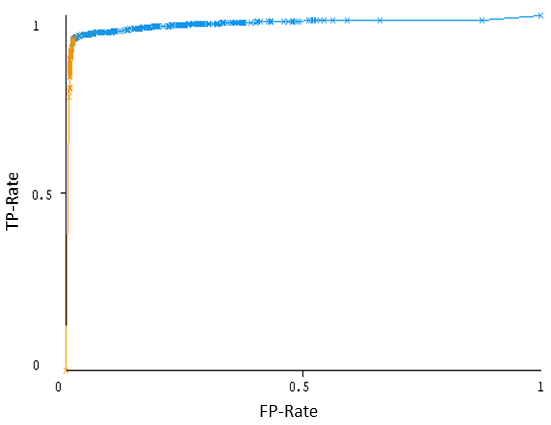
\includegraphics[width=0.25\linewidth]{images/j48_eval}} 
  \subfloat[][J48 erw.\\AUC = 0,61]{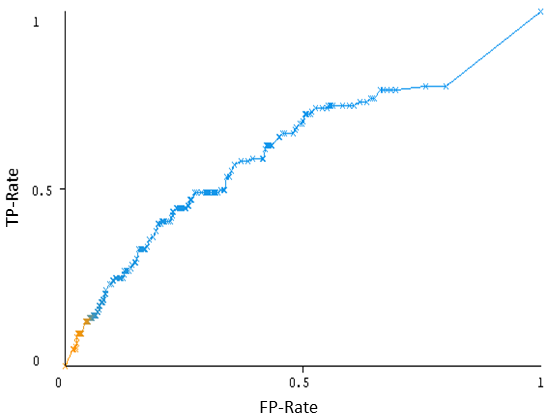
\includegraphics[width=0.25\linewidth]{images/j48_eval_feat}}
  \subfloat[][NN einf.\\AUC = 0,37]{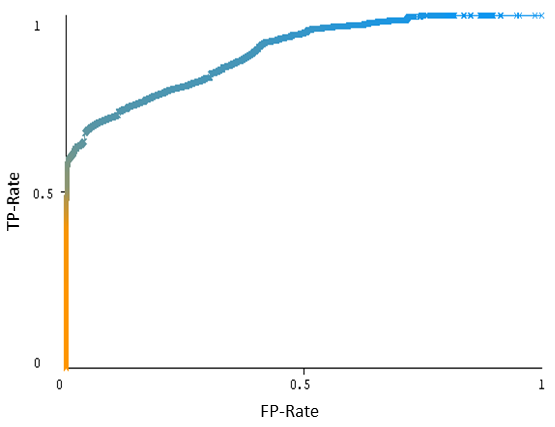
\includegraphics[width=0.25\linewidth]{images/nn_eval}}
  \subfloat[][NN erw.\\AUC = 0,54]{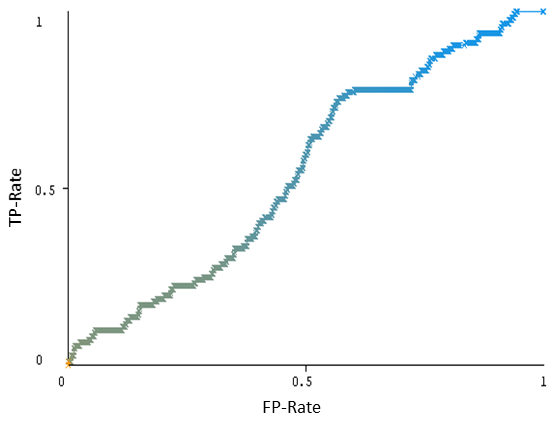
\includegraphics[width=0.25\linewidth]{images/nn_eval_feat}}
  \qquad
  \subfloat[][KNN einf.\\AUC = 0,55]{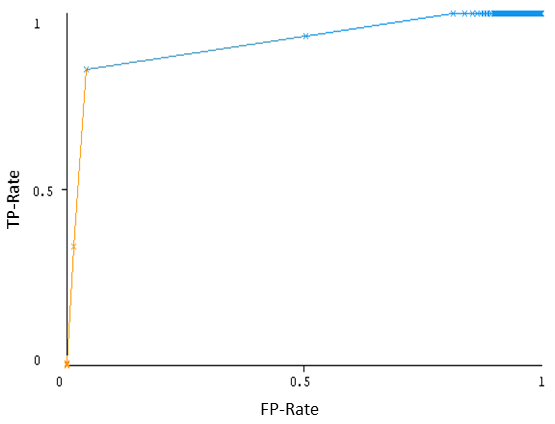
\includegraphics[width=0.25\linewidth]{images/knn_eval}}
  \subfloat[][KNN erw.\\AUC = 0,52]{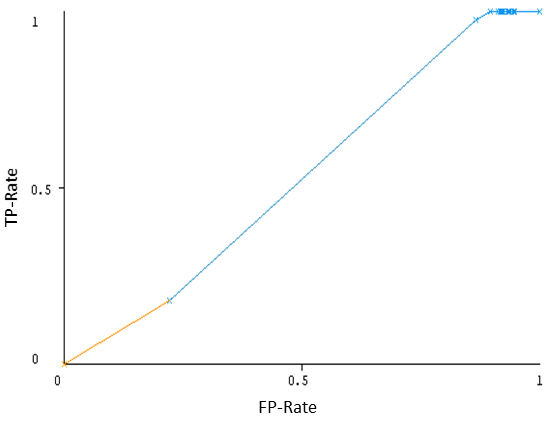
\includegraphics[width=0.25\linewidth]{images/knn_eval_feat}}
  \subfloat[][RF einf.\\AUC = 0,71]{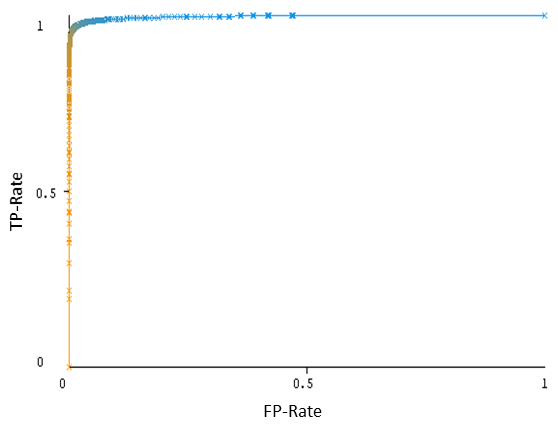
\includegraphics[width=0.25\linewidth]{images/rf_eval}} 
  \subfloat[][RF erw.\\AUC = 0,71]{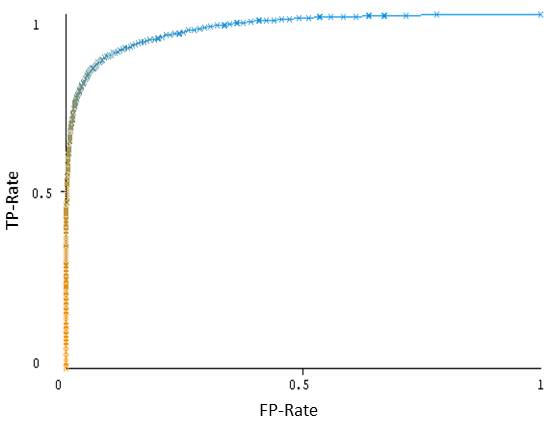
\includegraphics[width=0.25\linewidth]{images/rf_eval_feat}} 
  \qquad
  \subfloat[][LR einf.\\AUC = 0,65]{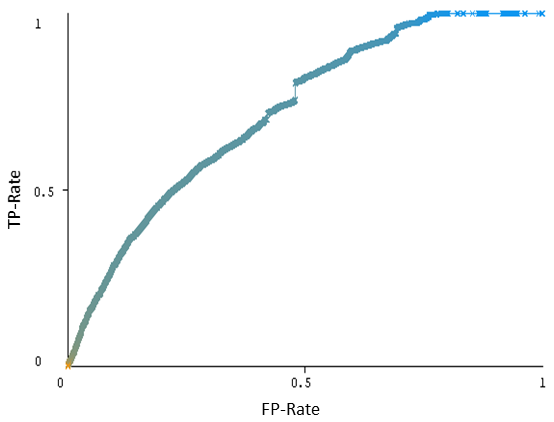
\includegraphics[width=0.25\linewidth]{images/lr_eval}}
  \subfloat[][LR erw.\\AUC = 0,62]{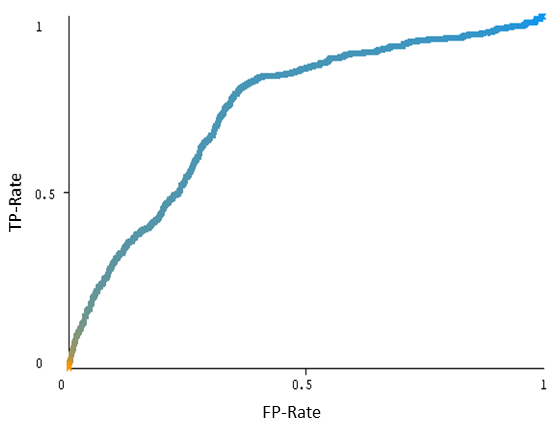
\includegraphics[width=0.25\linewidth]{images/lr_eval_feat}}
  \subfloat[][SGD einf.\\AUC = 0,57]{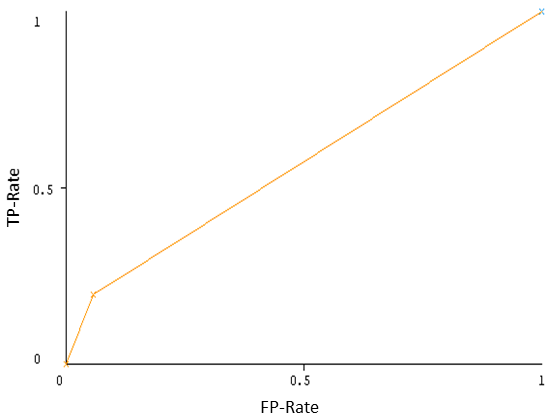
\includegraphics[width=0.25\linewidth]{images/sgd_eval}}
  \subfloat[][SGD erw.\\AUC = 0,56]{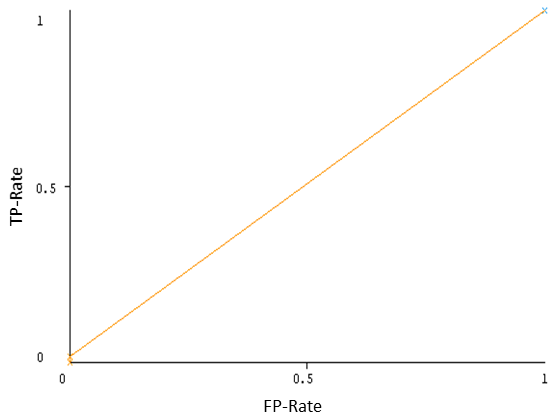
\includegraphics[width=0.25\linewidth]{images/sgd_eval_feat}}
  \qquad
  \subfloat[][NB einf.\\AUC = 0,48]{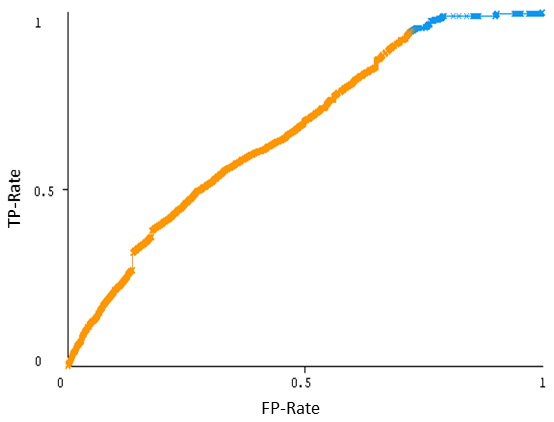
\includegraphics[width=0.25\linewidth]{images/nb_eval}}
  \subfloat[][NB erw.\\AUC = 0,47]{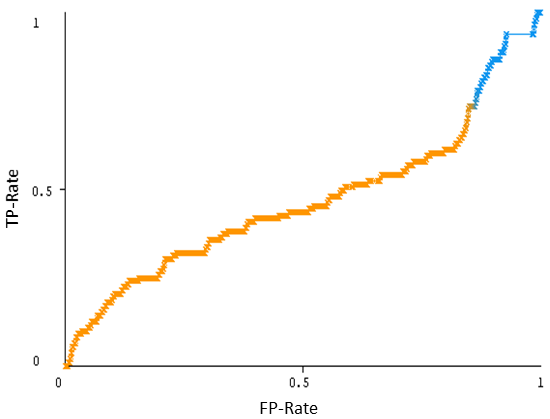
\includegraphics[width=0.25\linewidth]{images/nb_eval_feat}}
  \subfloat[][SVM einf.\\AUC = 0,57]{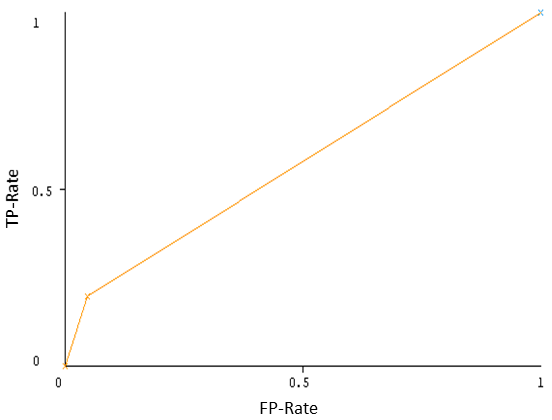
\includegraphics[width=0.25\linewidth]{images/svm_eval}}
  \subfloat[][SVM erw.\\AUC = 0,57]{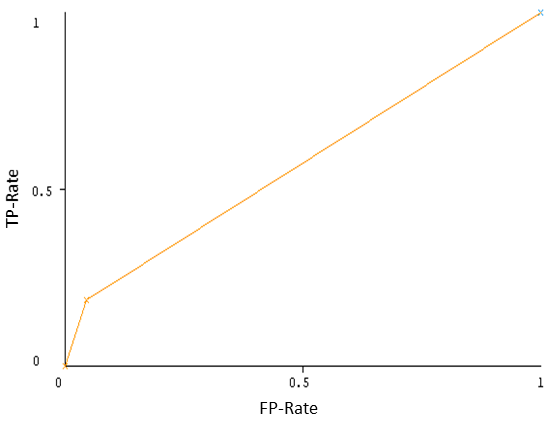
\includegraphics[width=0.25\linewidth]{images/svm_eval_feat}}
  \caption{ROC-Kurven der datenbasierten Datensets \label{roc-file}}
\end{figure}

\subsubsection*{Zusammenfassung}
Die Ergebnisse sämtlicher Metriken zeigten ein undifferenziertes und undeutliches Bild der Performanz der Klassifikatoren je Datenset. Der Grund für die gezeigten Ergebnisse ist die Unbalanciertheit der jeweiligen Testdatensets mit einem Anteil von \glqq defekt\grqq -Instanzen von 1\%. Damit für dieses Label gute Ergebnisse erzielt werden können, müssen viele korrekte Vorhersagen der Klassifikatoren getroffen werden. Dies war jedoch für das vorhandene Testdatenset nicht der Fall, sodass viele Vorhersagen fälschlicherweise dem dominierenden Label \glqq fehlerfrei\grqq{} zugeordnet wurden, die dann allerdings infolgedessen hohe FP-Raten aufweisen. Diesen Umstand spiegeln auch die Mittelwerte in \autoref{tab:met-results} wider. Aufgrund der deutlich schwächeren Werte der \glqq defekt\grqq -Spalten, werden die Gesamtwerte, die durch den Mittelwert repräsentiert werden, nach unten beeinflusst. Wie jedoch schon in \hyperref[smote]{Abschnitt 4.2} erläutert wurde, ist es nicht vorgesehen, die Unbalanciertheit der Testdatensets mithilfe des SMOTE-Algorithmus auszugleichen.

Um ein differenzierteres Bild der Performanz der Klassifikatoren zu erhalten, wurde eine weitere Testmethode, als Alternative zur Aufteilung der Datensets in Training- und Testdaten, hinzugezogen. Dabei handelt es sich um die sogenannte \glqq n-fold-cross-validation\grqq. Bei dieser Methode werden die Trainingsdaten in \texttt{n} gleich große Datenmengen (\glqq folds\grqq) aufgeteilt, welche dann jeweils mit einer Split-Ratio von 90:10 zum Training der einzelnen Klassifikatoren dienen \cite{IanWitten}. Die Ergebnisse der Evaluationsmetriken bilden sich dann aus dem Mittelwert der Einzelergebnisse der \texttt{n} Vorgänge \cite{IanWitten}. Diese Methode findet auch in der wissenschaftlichen Literatur Anwendung (zum Beispiel \cite{Alam2013,Chawla2002,Alsaeedi2019}. In diesem Fall wird eine 10-fold-cross-validation durchgeführt. Die Ergebnisse der Evaluationsmetriken sind in \autoref{tab:kx} aufgeführt. Ein Überblick über die Ergebnisse zeigt, dass diese wesentlich differenzierter und nachvollziehbarer ausgefallen sind sowie keine signifikanten Unterschiede zwischen den Datensets aufweisen. Es zeigt sich, dass die beiden Entscheidungsbaum-basierten Klassifikatoren J48 und RF die im Vergleich höchste Performanz mit einer Accuracy von 96\% beziehungsweise 98\% besitzen. Die FP-Rate der Klassifikatoren ist außerdem äußerst gering. Gleiches zeigt sich für den KNN-Klassifikator. Die weiteren Ergebnisse der Metriken bestätigen die hohe Performanz. Die Klassifikatoren SGD und SVM zeigen anhand ihrer ROC-Bereiche (siehe ROC-Area), dass sie unerwünschte Vorhersagen in Form des \glqq Ratens\grqq{} durchführen. Auffällig ist, dass die Werte zwischen den NN-Klassifikatoren beider Datensets nicht mehr abweichen. Beide Klassifikatoren arbeiten wie die weiteren, bisher unerwähnten, Klassifikatoren auf einem durchschnittlichen Niveau.

\begin{table}[ht]
\centering
\caption{Ergebnisse der Evaluationsmetriken auf Basis der 10-fold-cross-validation (TPR = TP-Rate, Rec. = Recall)}
\label{tab:kx}
\resizebox{\linewidth}{!}{%
\begin{tabular}{|>{\hspace{0pt}}p{0.06\linewidth}>{\hspace{0pt}}p{0.119\linewidth}|>{\RaggedLeft\hspace{0pt}}p{0.123\linewidth}>{\RaggedLeft\hspace{0pt}}p{0.17\linewidth}>{\RaggedLeft\hspace{0pt}}p{0.112\linewidth}|>{\RaggedLeft\hspace{0pt}}p{0.121\linewidth}>{\RaggedLeft\hspace{0pt}}p{0.168\linewidth}>{\RaggedLeft\hspace{0pt}}p{0.112\linewidth}|} 
\cline{3-8}
\multicolumn{1}{>{\hspace{0pt}}p{0.06\linewidth}}{} &           & \multicolumn{3}{>{\Centering\hspace{0pt}}p{0.405\linewidth}|}{\textbf{\glqq einfaches\grqq{} dateibasiertes Datenset} } & \multicolumn{3}{>{\Centering\hspace{0pt}}p{0.401\linewidth}|}{\textbf{erweitertes dateibasiertes Datenset} }  \\ 
\cline{3-8}
\multicolumn{1}{>{\hspace{0pt}}p{0.06\linewidth}}{} &           & \textbf{defekt}  & \textbf{fehlerfrei}                                 & \textbf{Mittel}                     & \textbf{defekt}  & \textbf{fehlerfrei}                                 & \textbf{Mittel}                      \\ 
\hline
\multirow{6}{0.06\linewidth}{\hspace{0pt}J48}       & Accuracy  & \multicolumn{2}{>{\RaggedLeft\hspace{0pt}}p{0.293\linewidth}}{gesamt:} & 0,96                                & \multicolumn{2}{>{\RaggedLeft\hspace{0pt}}p{0.289\linewidth}}{gesamt:} & 0,96                                 \\
                                                    & TPR/Rec.  & 0,94             & 0,97                                                & 0,96                                & 0,94             & 0,97                                                & 0,96                                 \\
                                                    & FP-Rate   & 0,03             & 0,06                                                & 0,05                                & 0,03             & 0,06                                                & 0,05                                 \\
                                                    & Precision & 0,96             & 0,96                                                & 0,96                                & 0,96             & 0,96                                                & 0,86                                 \\
                                                    & F-Score   & 0,95             & 0,97                                                & 0,96                                & 0,95             & 0,96                                                & 0,96                                 \\
                                                    & ROC-Area  & 0,97             & 0,97                                                & 0,97                                & 0,97             & 0,97                                                & 0,97                                 \\ 
\hline
\multirow{6}{0.06\linewidth}{\hspace{0pt}KNN}       & Accuracy  & \multicolumn{2}{>{\RaggedLeft\hspace{0pt}}p{0.293\linewidth}}{gesamt:} & 0,91                                & \multicolumn{2}{>{\RaggedLeft\hspace{0pt}}p{0.289\linewidth}}{gesamt:} & 0,91                                 \\
                                                    & TPR/Rec.  & 0,87             & 0,94                                                & 0,91                                & 0,87             & 0,94                                                & 0,91                                 \\
                                                    & FP-Rate   & 0,06             & 0,13                                                & 0,10                                & 0,06             & 0,13                                                & 0,10                                 \\
                                                    & Precision & 0,92             & 0,91                                                & 0,92                                & 0,91             & 0,91                                                & 0,91                                 \\
                                                    & F-Score   & 0,89             & 0,93                                                & 0,91                                & 0,89             & 0,92                                                & 0,91                                 \\
                                                    & ROC-Area  & 0,93             & 0,93                                                & 0,93                                & 0,93             & 0,93                                                & 0,93                                 \\ 
\hline
\multirow{6}{0.06\linewidth}{\hspace{0pt}LR}        & Accuracy  & \multicolumn{2}{>{\RaggedLeft\hspace{0pt}}p{0.293\linewidth}}{gesamt:} & 0,65                                & \multicolumn{2}{>{\RaggedLeft\hspace{0pt}}p{0.289\linewidth}}{gesamt:} & 0,65                                 \\
                                                    & TPR/Rec.  & 0,34             & 0,88                                                & 0,61                                & 0,35             & 0,87                                                & 0,61                                 \\
                                                    & FP-Rate   & 0,12             & 0,66                                                & 0,39                                & 0,13             & 0,65                                                & 0,39                                 \\
                                                    & Precision & 0,66             & 0,65                                                & 0,66                                & 0,66             & 0,66                                                & 0,66                                 \\
                                                    & F-Score   & 0,45             & 0,75                                                & 0,60                                & 0,46             & 0,75                                                & 0,61                                 \\
                                                    & ROC-Area  & 0,74             & 0,74                                                & 0,74                                & 0,74             & 0,74                                                & 0,74                                 \\ 
\hline
\multirow{6}{0.06\linewidth}{\hspace{0pt}NB}        & Accuracy  & \multicolumn{2}{>{\RaggedLeft\hspace{0pt}}p{0.293\linewidth}}{gesamt:} & 0,52                                & \multicolumn{2}{>{\RaggedLeft\hspace{0pt}}p{0.289\linewidth}}{gesamt:} & 0,52                                 \\
                                                    & TPR/Rec.  & 0,93             & 0,23                                                & 0,58                                & 0,94             & 0,22                                                & 0,58                                 \\
                                                    & FP-Rate   & 0,77             & 0,07                                                & 0,42                                & 0,78             & 0,06                                                & 0,42                                 \\
                                                    & Precision & 0,46             & 0,83                                                & 0,65                                & 0,46             & 0,84                                                & 0,65                                 \\
                                                    & F-Score   & 0,62             & 0,36                                                & 0,49                                & 0,62             & 0,35                                                & 0,49                                 \\
                                                    & ROC-Area  & 0,65             & 0,65                                                & 0,65                                & 0,65             & 0,65                                                & 0,65                                 \\ 
\hline
\multirow{6}{0.06\linewidth}{\hspace{0pt}NN}        & Accuracy  & \multicolumn{2}{>{\RaggedLeft\hspace{0pt}}p{0.293\linewidth}}{gesamt:} & 0,71                                & \multicolumn{2}{>{\RaggedLeft\hspace{0pt}}p{0.289\linewidth}}{gesamt:} & 0,70                                 \\
                                                    & TPR/Rec.  & 0,55             & 0,82                                                & 0,69                                & 0,54             & 0,82                                                & 0,68                                 \\
                                                    & FP-Rate   & 0,18             & 0,45                                                & 0,32                                & 0,18             & 0,46                                                & 0,32                                 \\
                                                    & Precision & 0,69             & 0,72                                                & 0,71                                & 0,68             & 0,72                                                & 0,70                                 \\
                                                    & F-Score   & 0,71             & 0,77                                                & 0,74                                & 0,60             & 0,76                                                & 0,68                                 \\
                                                    & ROC-Area  & 0,78             & 0,78                                                & 0,78                                & 0,79             & 0,79                                                & 0,79                                 \\ 
\hline
\multirow{6}{0.06\linewidth}{\hspace{0pt}RF}        & Accuracy  & \multicolumn{2}{>{\RaggedLeft\hspace{0pt}}p{0.293\linewidth}}{gesamt:} & 0,98                                & \multicolumn{2}{>{\RaggedLeft\hspace{0pt}}p{0.289\linewidth}}{gesamt:} & 0,98                                 \\
                                                    & TPR/Rec.  & 0,97             & 0,99                                                & 0,98                                & 0,97             & 0,99                                                & 0,98                                 \\
                                                    & FP-Rate   & 0,01             & 0,04                                                & 0,3                                 & 0,01             & 0,03                                                & 0,2                                  \\
                                                    & Precision & 0,98             & 0,98                                                & 0,98                                & 0,98             & 0,98                                                & 0,98                                 \\
                                                    & F-Score   & 0,97             & 0,98                                                & 0,98                                & 0,97             & 0,98                                                & 0,98                                 \\
                                                    & ROC-Area  & 0,99             & 0,99                                                & 0,99                                & 1,00             & 1,00                                                & 1,00                                 \\ 
\hline
\multirow{6}{0.06\linewidth}{\hspace{0pt}SGD}       & Accuracy  & \multicolumn{2}{>{\RaggedLeft\hspace{0pt}}p{0.293\linewidth}}{gesamt:} & 0,63                                & \multicolumn{2}{>{\RaggedLeft\hspace{0pt}}p{0.289\linewidth}}{gesamt:} & 0,63                                 \\
                                                    & TPR/Rec.  & 0,19             & 0,94                                                & 0,57                                & 0,18             & 0,94                                                & 0,56                                 \\
                                                    & FP-Rate   & 0,06             & 0,81                                                & 0,44                                & 0,06             & 0,82                                                & 0,44                                 \\
                                                    & Precision & 0,69             & 0,62                                                & 0,66                                & 0,69             & 0,62                                                & 0,66                                 \\
                                                    & F-Score   & 0,30             & 0,75                                                & 0,53                                & 0,29             & 0,75                                                & 0,52                                 \\
                                                    & ROC-Area  & 0,57             & 0,57                                                & 0,57                                & 0,56             & 0,56                                                & 0,56                                 \\ 
\hline
\multirow{6}{0.06\linewidth}{\hspace{0pt}SVM}       & Accuracy  & \multicolumn{2}{>{\RaggedLeft\hspace{0pt}}p{0.293\linewidth}}{gesamt:} & 0,62                                & \multicolumn{2}{>{\RaggedLeft\hspace{0pt}}p{0.289\linewidth}}{gesamt:} & 0,62                                 \\
                                                    & TPR/Rec.  & 0,16             & 0,95                                                & 0,56                                & 0,15             & 0,95                                                & 0,55                                 \\
                                                    & FP-Rate   & 0,05             & 0,84                                                & 0,45                                & 0,05             & 0,85                                                & 0,46                                 \\
                                                    & Precision & 0,69             & 0,62                                                & 0,66                                & 0,69             & 0,61                                                & 0,66                                 \\
                                                    & F-Score   & 0,26             & 0,75                                                & 0,51                                & 0,25             & 0,75                                                & 0,50                                 \\
                                                    & ROC-Area  & 0,55             & 0,55                                                & 0,55                                & 0,55             & 0,55                                                & 0,55                                 \\
\hline
\end{tabular}
}
\end{table}

Zusammenfassend lässt sich anhand der Ergebnisse beider Tests feststellen, dass der Einbezug der featurebasierten Metriken keinen nennenswerten positiven Einfluss auf die Ergebnisse der dateibasierten Fehlervorhersage besitzt. Hinzugefügt werden muss jedoch, dass sie die Ergebnisse auch nicht negativ beeinflussen. Ein Grund dafür ist, dass die Auswahl an Attributen für beide dateibasierten Datensets sehr hoch ist. Das \glqq einfache\grqq{} Datenset umfasst 17 Attribute (+ Label) und das erweiterte Datenset umfasst 28 Attribute (+ Label). Eine Reduzierung der Attribute in Form einer Attributsauswahl könnte dazu beitragen, den Einfluss der featurebasierten näher zu analysieren. Die Attributsauswahl beschreibt einen automatisierten Prozess, welcher dazu dient, die optimale Anzahl und Auswahl von Attributen für das Training eines Klassifikators zu bestimmen. Eine solche Funktion bietet das für die Arbeit verwendete Werkzeug WEKA. Die Autoren einer wissenschaftlichen Arbeit, die sich mit Codemetriken als Attributen zur Fehlervorhersage beschäftigte, kam zu dem Resultat, dass bereits drei Attribute ausreichend seien \cite{Wang2011}. Eine exemplarisch durchgeführte Attributsauswahl der Klassifikatoren LR, NB und SGD des erweiterten dateibasierten Datensets in der WEKA Workbench\footnote{Eine Attributsauswahl der weiteren Klassifikatoren des erweiterten dateibasierten Datensets wurde eingeleitet, konnte jedoch auch nach über zwölf Stunden Laufzeit nicht abgeschlossen werden und wurde daraufhin abgebrochen und nicht weiter nachverfolgt.} kam zu dem Ergebnis, welches in \autoref{tab:attribute-selection} aufgeführt sind. Die fettgedruckten Attribute der Spalte der ausgewählten Attribute entstammen dabei dem featurebasierten Datenset. Anhand dessen ist zu erkennen, dass nur höchstens 25\% der Attribute dieses Datensets ausgewählt wurden. Dies zeigt ebenfalls, dass die featurebasierten Metriken, die das \glqq einfache\grqq{} dateibasierte Datenset erweitern, nur einen geringen Einfluss auf die Vorhersagen aufweisen.

\begin{table}[ht]
\centering
\caption{Ergebnisse der Attributsauswahl der Klassifikatoren LR, NB und SGD }
\label{tab:attribute-selection}
\resizebox{\linewidth}{!}{%
\begin{tabular}{|l|l|l|} 
\hline
\textbf{Klassifikator} & \textbf{ausgewählte Attribute}                                                                                                    & \textbf{abgelehnte Attribute}                                                                                                                                                                         \\ 
\hline
LR                     & \begin{tabular}[c]{@{}l@{}} \texttt{\textbf{MODS}}, \texttt{\textbf{FADDL}}*, \texttt{\textbf{FREML}}*, \texttt{BUGF},\\\texttt{AUTH}, \texttt{ADDL}, \texttt{REML}, \texttt{CCHL},\\\texttt{CCHM}, \texttt{CCHA}, \texttt{AVGC}, \texttt{WAGE}\\(12 von 28)\end{tabular} & \begin{tabular}[c]{@{}l@{}}\texttt{COMM}, \texttt{ADEV}, \texttt{DDEV}, \texttt{EXP},\\\texttt{OEXP}, \texttt{MODD}, \texttt{NLOC}, \texttt{CYCO},\\\texttt{REVI}, \texttt{REFA}, \texttt{ADDM}, \texttt{ADDA},\\\texttt{REMM}, \texttt{REMA}, \texttt{MAXC}, \texttt{AAGE}\\(16 von 28)\end{tabular}                                                 \\ 
\hline
NB                     & \begin{tabular}[c]{@{}l@{}}\texttt{\textbf{MODS}}, \texttt{BUGF}, \texttt{AUTH}, \texttt{CCHM},\\\texttt{WAGE} (5 von 28)\end{tabular}                                                  & \begin{tabular}[c]{@{}l@{}}\texttt{COMM}, \texttt{ADEV}, \texttt{DDEV}, \texttt{EXP},\\\texttt{OEXP}, \texttt{MODD}, \texttt{NLOC}, \texttt{CYCO},\\\texttt{FADDL}*, \texttt{FREML}*, \texttt{REVI}, \texttt{REFA},\\\texttt{ADDL}, \texttt{ADDM}, \texttt{ADDA}, \texttt{REML},\\\texttt{REMM}, \texttt{REMA}, \texttt{CCHL}, \texttt{CCHA},\\\texttt{MAXC}, \texttt{AVGC}, \texttt{AAGE} (23 von 28)\end{tabular}  \\ 
\hline
SGD                    & \begin{tabular}[c]{@{}l@{}}\texttt{\textbf{MODS}}, \texttt{\textbf{FREML}}*, \texttt{REVI}, \texttt{REFA}\\\texttt{BUGF}, \texttt{AUTH}, \texttt{CCHM}, \texttt{CCHA},\\\texttt{AVGC}, \texttt{AAGE}, \texttt{WAGE} (11 von 28)\end{tabular}           & \begin{tabular}[c]{@{}l@{}}\texttt{COMM}, \texttt{ADEV}, \texttt{DDEV}, \texttt{EXP},\\\texttt{OEXP}, \texttt{MODD}, \texttt{NLOC}, \texttt{CYCO},\\\texttt{FADDL}*, \texttt{ADDL}, \texttt{ADDM}, \texttt{ADDA},\\\texttt{REML}, \texttt{REMM}, \texttt{REMA}, \texttt{CCHL},\\\texttt{MAXC} (17 von 28)\end{tabular}                                         \\ 
\hline
\multicolumn{3}{|c|}{* ADDL- und REML-Metriken des featurebasierten Datensets}                                                                                                                                                                                                                                                                                      \\
\hline
\end{tabular}
}
\end{table}

\fbox{\parbox{\linewidth}{RQ3c: WIE LASSEN SICH DIE KLASSIFIKATOREN MIT WEITEREN VORHERSAGETECHNIKEN, DIE KEINE FEATURES NUTZEN, VERGLEICHEN?\medskip\\
Es wurde auf eine Methode zur Erstellung eines dateibasierten Datensets aus der wissenschaftlichen Literatur zurückgegriffen \cite{Moser2008}. Dieses Datenset basiert auf den mittels PyDriller abgerufenen Daten und umfasst 17 Prozessmetriken als Attribute. Zum besseren Vergleich wurde ein zusätzliches erweitertes dateibasiertes Datenset erstellt, welches die selben Prozessmetriken, aber auch zusätzlich die featurebasierten Metriken auf Dateiebene gemapped, umfasst.}}

\fbox{\parbox{\linewidth}{RQ3d: WIE BEEINFLUSST DIE VERWENDUNG VON FEATUREBASIERTEN METRIKEN DIE FEHLERVORHERSAGE?\medskip\\
Die Auswirkungen des Einbezugs der featurebasierten Metriken sind kaum messbar. Sowohl die Klassifikatoren des \glqq einfachen\grqq{} dateibasierten Datensets als auch die des erweiterten dateibasierten Datensets, erzielen die selben Ergebnisse mit geringen Abweichungen. Sie sind somit jeweils gleich performant bezüglich der Vorhersagen.}}

\cleardoublepage